\documentclass[12pt,a4paper]{article}

\renewcommand*\contentsname{Sadržaj}
\renewcommand{\figurename}{Slika}
\renewcommand{\tablename}{Tabela}
\renewcommand\refname{Reference}
\renewcommand{\arraystretch}{1.25}

\usepackage[margin=0.85in]{geometry}
\usepackage{graphicx}
\usepackage{float}
\usepackage{listings}
\usepackage{multirow}
\usepackage[table]{xcolor}
\usepackage{colortbl}
\usepackage{color}
\usepackage{hyperref}
\usepackage{ctable}
\usepackage{array}
\usepackage{hhline}
\usepackage{caption}
\usepackage{amsfonts}
\usepackage{flowchart}
\usepackage{enumitem}
\usepackage{mathabx}
\usepackage{amssymb}
\usepackage{titlesec}
\usetikzlibrary{arrows}

\lstloadlanguages{C,C++,csh,Java}

\definecolor{red}{rgb}{0.6,0,0} 
\definecolor{blue}{rgb}{0,0,0.6}
\definecolor{green}{rgb}{0,0.8,0}
\definecolor{cyan}{rgb}{0.0,0.6,0.6}
\definecolor{magnolia}{rgb}{0.97, 0.96, 1.0}
\definecolor{colora}{rgb}{0.67, 0.8, 0.94}
\definecolor{colorb}{rgb}{0.67, 0.94, 0.82}
\definecolor{colord}{rgb}{0.67, 0.9, 0.93}
\definecolor{colore}{rgb}{0.6, 0.73, 0.89}
\definecolor{colorf}{rgb}{0.61, 0.87, 1.0}
\definecolor{grey}{rgb}{0.75, 0.75, 0.75}
\definecolor{amber}{rgb}{1.0, 0.75, 0.0}

\lstset{
language=csh,
basicstyle=\footnotesize\ttfamily,
numbers=left,
numberstyle=\tiny,
numbersep=5pt,
tabsize=2,
extendedchars=true,
breaklines=true,
frame=b,
stringstyle=\color{blue}\ttfamily,
showspaces=false,
showtabs=false,
xleftmargin=17pt,
framexleftmargin=17pt,
framexrightmargin=5pt,
framexbottommargin=4pt,
commentstyle=\color{green},
morecomment=[l]{//}, %use comment-line-style!
morecomment=[s]{/*}{*/}, %for multiline comments
showstringspaces=false,
morekeywords={ abstract, event, new, struct,
as, explicit, null, switch,
base, extern, object, this,
bool, false, operator, throw,
break, finally, out, true,
byte, fixed, override, try,
case, float, params, typeof,
catch, for, private, uint,
char, foreach, protected, ulong,
checked, goto, public, unchecked,
class, if, readonly, unsafe,
const, implicit, ref, ushort,
continue, in, return, using,
decimal, int, sbyte, virtual,
default, interface, sealed, volatile,
delegate, internal, short, void,
do, is, sizeof, while,
double, lock, stackalloc,
else, long, static,
enum, namespace, string},
keywordstyle=\color{cyan},
identifierstyle=\color{red},
backgroundcolor=\color{magnolia},
}

\DeclareCaptionFont{white}{\color{white}}
\DeclareCaptionFormat{listing}{\colorbox{blue}{\parbox{\textwidth}{\hspace{15pt}#1#2#3}}}
\captionsetup[lstlisting]{format=listing,labelfont=white,textfont=white, singlelinecheck=false, margin=0pt, font={bf,footnotesize}}

\newcolumntype{a}{>{\columncolor{colora}}c}
\newcolumntype{b}{>{\columncolor{colorb}}c}
\newcolumntype{d}{>{\columncolor{colord}}c}
\newcolumntype{e}{>{\columncolor{colore}}c}
\newcolumntype{f}{>{\columncolor{colorf}}c}
\newcolumntype{P}[1]{>{\centering\arraybackslash}p{#1}}
\newcolumntype{?}{!{\vrule width 1pt}}

\begin{document}

\begin{titlepage}
	\centering
	{\scshape Univerzitet u Sarajevu \par}
	{\scshape Elektrotehnički Fakultet \par}
	{\scshape Odsjek za Računarstvo i Informatiku \par}
	\vspace{2cm}
	{\Large\scshape Praktikum: Poslovni Informacioni Sistemi\par}
	\vspace{2.5cm}
	{\huge\bfseries \textit{Service Requirements Specification} Dokument\par}
	\vspace{2.5cm}
	\Large Studenti: \par
	{\Large\itshape \textsc{Bojadžić} Hanna, 1421/17311\par}
	{\Large\itshape \textsc{Građanin} Ehvan, 1438/17335\par}
	{\Large\itshape \textsc{Halilbegović} Kemal, 1469/16682\par}
	{\Large\itshape \textsc{Krupalija} Ehlimana, 1431/17461\par}
	{\Large\itshape \textsc{Kubat} Ismar, 1422/17148\par}
	{\Large\itshape \textsc{Kulović} Nejra, 1519/17484\par}
	{\Large\itshape \textsc{Muftić} Belma, 1423/17260\par}
	{\Large\itshape \textsc{Pribišić} Tarik, 1536/2018\par}
	\vfill
	Predmetni nastavnik:\par
	doc. dr. \textsc{Anel Tanović}, dipl. ing. el.
	\vfill
	{\large Juni, 2019\par}
\end{titlepage}

\pagenumbering{gobble}

\tableofcontents

\newpage

\pagenumbering{arabic}

\section{ITIL procesi}

\subsection{\textit{Change Management}}

\quad Upravljanje promjenama je ITIL (\textit{Information Technology Infrastructure Library}) proces koji pripada skupu procesa u okviru tranzicije usluga. Njegova svrha je upravljanje promjenama koje se dešavaju nad nekim IT servisom, te olakšavanje prilagođavanja promjenama, kao i njihovom uvođenju i što boljem procesiranju zahtjeva za promjenama. U prvim verzijama ITIL-a promjene su bile generičke, no u kasnijim verzijama (od verzije 3 nadalje) prepoznata je potreba za uvođenjem tzv. modela promjena, koji razdvajaju promjene u različite kategorije prema značaju i hitnosti.

Pri upravljanju promjenama potrebno je definisati sljedeće pojmove:

\begin{enumerate}
\item \textbf{Zahtjev za promjenom (\textit{Request for Change - RFC})} - trebaju postojati jasno definisani slučajevi u kojima se prepoznaje potreba za vršenjem promjena. Promjene mogu inicirati osobe od interesa (\textit{stakeholderi}, ukoliko je u pitanju IT usluga koju koristi neka kompanija i sl.), ili mogu biti vođene odzivom sistema, odnosno inicirane zbog grešaka, pogrešnog ili slabog korištenja nekih dijelova sistema. Zbog toga je važno omogućiti različitim osobama od interesa iniciranje promjena, kao i osigurati da se vrši praćenje korištenja sistema te analiza uspješnosti i frekvencije korištenja istog.

\item \textbf{Promjena} -  moguće je vršiti različite akcije nad sistemom koje se smatraju promjenom: dodavanje novih komponenti, izmjenu ili potpuno uklanjanje starih, spajanje različitih funkcionalnosti i mnoge druge. Različite vrste promjena trebaju se tretirati na različite načine. Potrebno je jasno definisati šta je moguća promjena, koja je njena kategorija, koliki je njen prioritet te ko je zadužen za implementaciju iste.

\item \textbf{Tim za upravljanje promjenama} - treba postojati jasno definisana uloga za osobe koje će moći nadzirati promjene, odobravati vršenje istih ili odbacivati prijedloge. Od ovog osoblja očekuje se da je u stanju brzo i adekvatno reagovati na hitne promjene, kao i da izvrši ispravno rasuđivanje da li će neka promjena pozitivno ili negativno utjecati na sam sistem (potrebno je izvršiti analizu koja se dokumentuje u vidu \textit{Projected Service Outage - PSO} dokumenta, u kojem su izlistane sve predvidljive devijacije od plana promjena).
\end{enumerate}

Upravljanje promjenama sastoji se od četiri osnovna podprocesa:

\begin{enumerate}
\item \textbf{Filtriranje promjena}, u okviru kojeg se pregledaju svi primljeni zahtjevi za vršenje promjena, analiziraju se i vrši se odluka koji zahtjevi će se prihvatiti, a koji zahtjevi će se odbiti, uz što se prilaže PSO dokument.

\item \textbf{Savjetovanje sa CAB (\textit{Change Advisory Board} i komitetom za hitne promjene}, što se odnosi na argumentovanje prethodno utvrđenih zahtjeva koji su prepoznati kao neophodni, te predstavljanje tih argumenata savjetima i komitetima koji jedini imaju autoritet za odobravanje promjena. Tek nakon što se promjene odobre, počinje se sa njihovom implementacijom. U svakom drugom slučaju, promjene se odbacuju.

\item \textbf{Upravljanje promjenama}, što se odnosi na dodjeljivanje posla zaposlenicima ovisno o vrsti zahtjeva koji je potrebno ispuniti te praćenje rada na dodavanju novih, zamjenom ili uklanjanjem postojećih funkcionalnosti u skladu s postojećim zahtjevima. Upravljanje promjenama vrši se stalno, od početka do kraja procesa njihovog uvođenja u sistem.

\item \textbf{Izvještavanje o promjenama}, odnosno kreiranje izvještaja o svakoj izvršenoj promjeni, što uključuje argumente za i protiv vršenja promjena, PSO dokument, dozvolu od CAB i drugih komiteta, kao i izvještaj o samom procesu implementacije i uvođenja promjena te kako je uvođenje istih u sistem promijenilo poslovanje, tj. da li je uvođenje promjena imalo pozitivan efekat ili ne.

\end{enumerate}

\subsection{\textit{Event Management}}

\quad Upravljanje događajima je ITIL (\textit{Information Technology Infrastructure Library}) proces koji pripada skupu procesa u okviru upravljanja uslugama. Njegova svrha je da nadzire sve značajne događaje u sistemu, detektuje nove i procesira ih na adekvatan način. Ovaj proces u \textit{ITIL}-u 2011 povezan je sa upravljanjem pristupom preko interfejsa, budući da su ta dva procesa u bliskoj korelaciji: u sistemu koji nadzire važne, često sigurnosno osjetljive događaje, onemogućavanje neautorizovanog pristupa jedan je od najvažnijih zahtjeva. \\

Pri upravljanju događajima potrebno je definisati sljedeće pojmove:

\begin{enumerate}
\item \textbf{Događaj} - u kompleksnim sistemima postoje različite vrste događaja i notifikacija, te je potrebno napraviti razgraničenje kojim vrstama događaja se bavi sistem upravljanjem događajima (događaji se najčešće dijele na informacije, upozorenja i greške).

\item \textbf{Prioritet} - različiti događaji imaju različit značaj, pri čemu je neke događaje potrebno hitno procesirati, dok drugi događaji mogu čekati određeno vrijeme. Iz tog razloga neophodno je svim vrstama događaja dodijeliti određene prioritete, koji se najčešće označavaju brojevima.

\item \textbf{Odziv} - sistem najčešće treba reagovati na događaje, posebno ukoliko je njihov prioritet veliki. Iz tog razloga potrebno je definisati vrstu i vrijeme odziva na različite događaje, te način njihovog procesiranja.
\end{enumerate}

Upravljanje događajima sastoji se od četiri osnovna podprocesa:

\begin{enumerate}
\item \textbf{Korištenje mehanizama za nadzor događaja}, koji se odnosi na stalnu mogućnost sistema da detektuje događaje, kao i da nadzire postojeće događaje i vrši njihovo procesiranje. Budući da je broj događaja koji konstantno ulaze u sistem veoma veliki, vrlo je važno ispravno izvršiti diferenciranje na različite vrste događaja, kako se ne bi detektovao veliki broj nevažnih ili nekritičnih događaja. S druge strane, sistem mora biti u mogućnosti reagovati na događaje na adekvatan način, posebno u slučaju kad se više različitih događaja treba procesirati u isto vrijeme.

\item \textbf{Prvi nivo korelacije: \textit{Filtriranje događaja}}, odnosno analiza događaja kako bi se odredilo da li je događaj relevantan za sistem ili ne. Ukoliko je događaj samo informacija, najčešće nije potrebno vršiti nikakve akcije te se takvi događaji mogu ignorisati. No, upozorenja i greške se moraju procesirati na adekvatan način, te je vrlo važno imati adekvatne mehanizme kako takvi događaji ne bi bili ignorisani (ali i kako informacije ne bi bile procesirane, ukoliko to nije neophodno).

\item \textbf{Drugi nivo korelacije: \textit{Izbor odziva}}, odnosno dalja analiza događaja koji nisu filtrirani na prethodnom nivou. Budući da je za upozorenja i greške najčešće potrebno imati adekvatan odziv, na ovom nivou potrebno je odrediti da li odziv može biti automatski (u pitanju je neki od poznatih događaja za koje postoje predefinisani koraci odziva), ili je potrebno eskalirati situaciju na viši nivo.

\item \textbf{Pregled događaja i njegovo zatvaranje}, koji se odnosi na dodatnu provjeru aktivnih događaja koji se trenutno nadziru. Ukoliko je automatska akcija bila dovoljna da se događaj procesira na adekvatan način i stanje vrati u normalno, te ukoliko je sistem proslijedio informacije o događaju individuama sistema koji su ga procesirali na adekvatan način, takav događaj moguće je zatvoriti, kako bi se novi događaji mogli procesirati bez čekanja.
\end{enumerate}

\newpage

\section{Opis i namjena sistema}

\subsection{Osnovne informacije o kompaniji}

\quad Kompanija \textbf{Idea d.o.o. Sarajevo} je mlada kompanija koja se bavi razvojem i održavanjem informacionih sistema za državne institucije, poput Zavoda za izgradnju Kantona Sarajevo, Zavoda za informatiku i statistiku Kantona Sarajevo, Direkcije za robne rezerve Kantona Sarajevo i mnogih drugih. Ovi informacioni sistemi omogućavaju pregled svih zaposlenika, njihovih personalnih dosijea (uključujući lične podatke, razne vrste dokumenata, rješenja i ugovora) te iniciranje različitih akcija, poput slanja na seminare, edukacije i stručna usavršavanja, vršenje ocjenjivanja radnika, donošenje različitih vrsta rješenja te vršenje sistematizacije. \\

Softver koji je razvijen potrebno je svakodnevno održavati. Korisnici sistema su najčešće srednje životne dobi, bez tehničkog znanja na visokom nivou, te se svakodnevno susreću s različitim poteškoćama u korištenju sistema. Ponekad dolazi do pojave grešaka, na koje je potrebno što prije reagovati, kako se ne bi ugrozilo ispravno i kontinualno funkcionisanje sistema. Same institucije često šalju zahtjeve za promjenama sistema, zbog stalnog donošenja novih odredbi te izmjene starih, zbog čega je sistem potrebno stalno ažurirati kako bi odgovarao trenutnom stanju i olakšavao poslovanje ovih instituacija. \\

Iz svih ovih razloga, Idea d.o.o. Sarajevo ima potrebu za razvojem aplikacije koja će im omogućiti upravljanje događajima i promjenama u sistemu. Ovakva aplikacija olakšati će detekciju grešaka i zahtjeva za promjenama, ubrzati reagovanje na hitne promjene te osigurati da sistem kontinualno funkcioniše bez problema, te da njegovi korisnici mogu imati pouzdano i ažurirano okruženje u kojem će im biti jednostavno raditi.

\subsection{Poslovni procesi}

\quad Kompanija želi informacioni sistem koji omogućava sljedeće funkcionalnosti:

\begin{itemize}
\renewcommand\labelitemi{$\square$}
\item Pregled svih zahtjeva za promjenama od strane tima za upravljanje promjenama;
\item Pisanje izvještaja (PSO dokumenta) o predloženoj promjeni te slanje istog komitetu za promjene na pregled;
\item Konačno odobravanje ili odbijanje promjena od strane komiteta za promjene;
\item Prihvatanje i odbijanje promjena, te njihovo označavanje kompletiranim nakon implementacije;
\item Slanje promjena timu za produkciju;
\item Prijavljivanje grešaka i problema pri implementaciji od strane tima za produkciju;
\item Pregled statističke analize korištenja sistema, uz informacije o slabo ili nikako korištenim dijelovima;
\item Prijava problema pri korištenju i slanje zahtjeva za promjene od strane korisnika sistema koji firma održava.
\end{itemize}

Sve ove funkcionalnosti trebaju biti objedinjene u jednoj aplikaciji, te mora biti osigurana sigurnost i konzistentnost podataka. U nastavku će biti prikazane osnovne informacije vezane za ITIL procese pomoću kojih je moguće modelirati poslovne procese sistema za koji je potrebno napraviti aplikaciju.

\subsubsection{Upravljanje promjenama}

\quad Sama svrha sistema je praćenje korištenja softvera koji se održava te prijem i procesiranje zahtjeva za promjene. U skladu s tim, definišu se dvije kategorije promjena:

\begin{itemize}
\renewcommand\labelitemi{-}
\item \textit{Obične promjene}, odnosno promjene koje inicijalizira tim za upravljanje promjenama na osnovu zahtjeva koje šalju autorizirani korisnici sistema koje firma Idea razvija i održava, ili koje tim za upravljanje promjenama ocijeni neophodnim na osnovu statističke analize korištenja sistema (slabo ili nikako korišteni dijelovi sistema);
\item \textit{Hitne promjene}, koje se detektuju na osnovu prijave problema pri korištenju od strane korisnika sistema koje firma održava. Prijava problema korisnicima je omogućena unutar same aplikacije.
\end{itemize}

Osim kategorija, promjene imaju i svoje vrste, kako slijedi:

\begin{itemize}
\renewcommand\labelitemi{-}
\item Dodavanje novih komponenti;
\item Izmjena postojećih komponenti;
\item Brisanje postojećih komponenti.
\end{itemize}

Svaka promjena mora imati definisanu kategoriju i vrstu. Tim za upravljanje promjenama vrši njihov pregled i filtriranje - zahtjev se analizira, te se ili odbija uz obrazloženje, ili se šalje komitetu za promjene na dodatnu analizu i odobravanje. Komitet za promjene ima mogućnost pregleda svih promjena koje su im poslane od strane tima za upravljanje promjenama, te odbijanje ili odobravanje promjena. Te informacije prosljeđuju se timu za upravljanje promjenama, te ukoliko se odobri vršenje promjena, iste se dodjeljuju jednom od dostupnih timova za razvoj softvera. \\

Na osnovu ovih informacija, moguće je dodijeliti određene funkcionalnosti sistema različitim vrstama korisnika, na način kako slijedi:

\begin{itemize}
\renewcommand\labelitemi{$\square$}
\item Slanje novog zahtjeva za promjenama - \textcolor{orange}{korisnici sistema};
\item Pregled svih zahtjeva za promjenama - \textcolor{blue}{tim za upravljanje promjenama};
\item Pisanje izvještaja (PSO dokumenta) o predloženoj promjeni te slanje istog komitetu za promjene na pregled - \textcolor{blue}{tim za upravljanje promjenama};
\item Prihvatanje i odbijanje promjena, te njihovo označavanje kompletiranim nakon implementacije - \textcolor{blue}{tim za upravljanje promjenama};
\item Konačno odobravanje ili odbijanje promjena - \textcolor{green}{komitet za promjene};
\item Slanje promjena timu za produkciju - \textcolor{blue}{tim za upravljanje promjenama};
\item Pregled statističke analize korištenja sistema, uz informacije o slabo ili nikako korištenim dijelovima - \textcolor{blue}{tim za upravljanje promjenama}.
\end{itemize}

\subsubsection{Upravljanje događajima}

\quad Događaje u sistemu predstavljaju prijave problema od strane korisnika sistema koji se održavaju, ili od strane razvojnog tima koji vrši implementaciju izmjena u sistemu. Pregled i nadziranje događaja vrši tim za upravljanje promjenama, dok korisnici sistema i razvojni tim mogu vršiti iniciranje novih događaja. \\

U skladu s ovim, potrebno je izvršiti definisanje svih različitih događaja u sistemu, njihovih tipova i prioriteta, što je prikazano u Tabeli \ref{tabela1}.

\begin{table}[H]
\centering
\begin{tabular}{| c | c | c |} \hline
\cellcolor{gray!25}\textbf{Vrsta događaja}		& \cellcolor{gray!25}\textbf{Inicijator}			& \cellcolor{gray!25}\textbf{Prioritet} 			\\ \hline
Greška u aplikaciji									& \cellcolor{green!25}Korisnik						& \cellcolor{blue!15}3							\\ \hline
Pogrešno korištenje aplikacije						& \cellcolor{green!25}Korisnik						& \cellcolor{blue!15}1							\\ \hline
Greška nakon uvođenja promjena					& \cellcolor{yellow!25}Razvojni tim				& \cellcolor{blue!35}2							\\ \hline
Nemogućnost implementacije promjene			& \cellcolor{yellow!25}Razvojni tim				& \cellcolor{blue!15}3							\\ \hline
\end{tabular}
\caption{Svi događaji sistema}
\label{tabela1}
\end{table}

Svi događaji prikazuju se timu za upravljanje promjenama, koji vrše odziv na događaje, na jedan od tri načina:

\begin{itemize}
\renewcommand\labelitemi{-}
\item \textit{Otkazivanje promjena}, koje se vrši ukoliko razvojni tim prijavi da nije u mogućnosti da implementira promjene iz nekog razloga (poput samog načina na koji sistem funkcioniše, nedovoljnog broja informacija o samoj promjeni koju je potrebno izvršiti, nemogućnosti povezivanja sa postojećim sistemom i sl.).
\item \textit{Slanje razvojnom timu na popravljanje}, koje se vrši ukoliko korisnici prijave grešku u sistemu prije ili nakon uvođenja promjena ili ukoliko dođe do greške pri testiranju sistema nakon uvođenja promjena.
\item \textit{Organizacija edukacije korisnika ili razgovor s korisnikom}, koji se vrše ukoliko korisnik prijavi da ne zna kako ispravno koristiti sistem, što nije dio samog sistema koji se razvija.
\end{itemize}

Na osnovu ovih informacija, moguće je dodijeliti određene funkcionalnosti sistema različitim vrstama korisnika, na način kako slijedi:

\begin{itemize}
\renewcommand\labelitemi{$\square$}
\item Prijavljivanje grešaka i problema pri implementaciji promjena - \textcolor{red}{razvojni tim};
\item Prijava problema pri korištenju sistema koji firma održava - \textcolor{brown}{korisnici sistema koji se održava}.
\end{itemize}

\newpage

\subsection{Pregled slučajeva upotrebe}

\quad Slučajevi upotrebe sistema koji odgovaraju funkcionalnostima vezanim za upravljanje promjenama prikazani su na Slici \ref{useCase1}. Akteri sistema su tim za upravljanje promjenama, komitet za promjene i tim za produkciju, koji učestvuju u realizaciji slučajeva upotrebe.

\begin{figure}[H]
\center
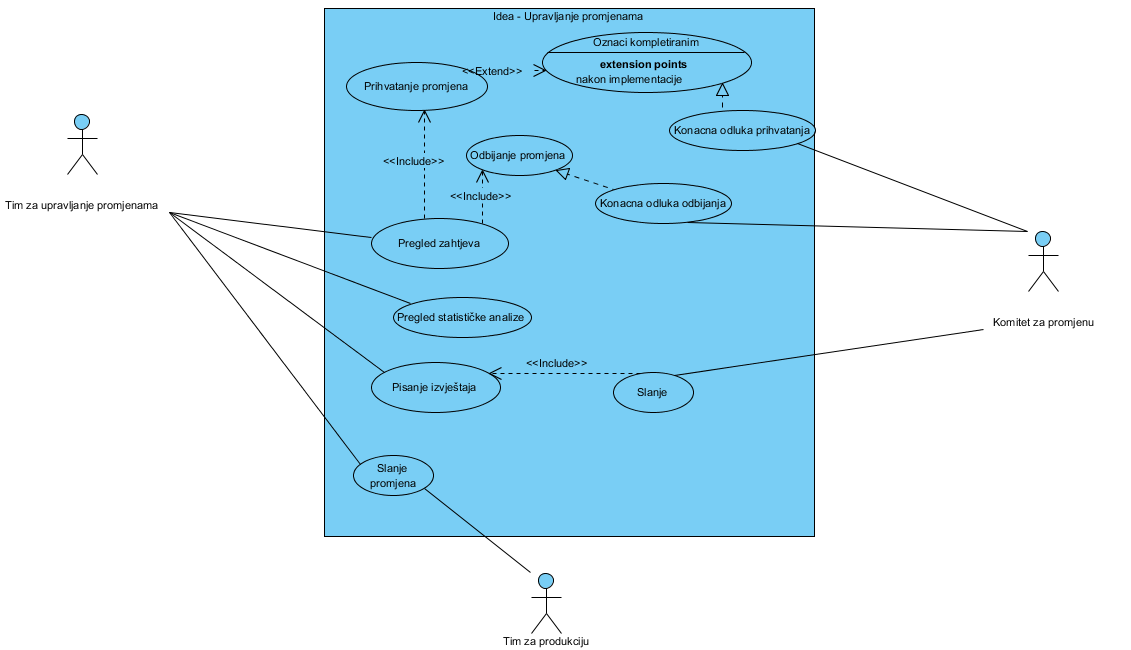
\includegraphics[scale=0.4]{../res/UseCase/useCase1.PNG}
\caption{Dijagram slučajeva upotrebe za upravljanje promjenama u sistemu}
\label{useCase1}
\end{figure}

Slučajevi upotrebe sistema koji odgovaraju funkcionalnostima vezanim za upravljanje događajima prikazani su na Slici \ref{useCase2}. Akteri sistema su korisnici sistema i tim za produkciju, koji učestvuju u realizaciji slučajeva upotrebe.

\begin{figure}[H]
\center
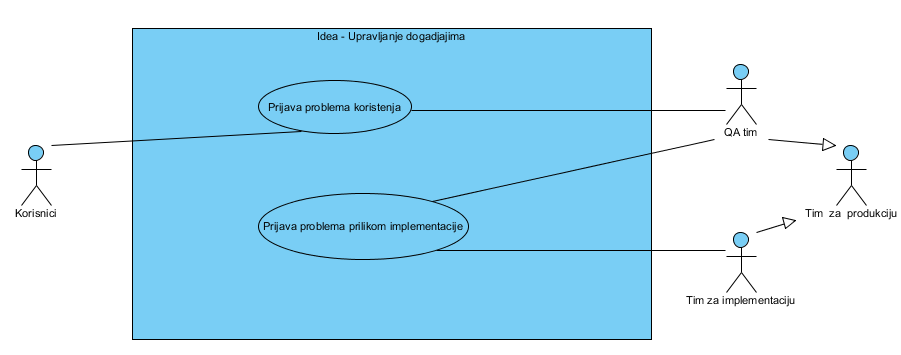
\includegraphics[scale=0.45]{../res/UseCase/useCase2.PNG}
\caption{Dijagram slučajeva upotrebe za upravljanje događajima u sistemu}
\label{useCase2}
\end{figure}

\newpage

\subsection{Metodologija razvoja sistema}

\quad Za razvoj sistema biti će korištena SCRUM metodologija, koja predstavlja jednu od najpoznatijih agilnih metodologija za razvoj softvera. Razvoj sistema obavljati će se u sprintovima, sa trajanjem svakog sprinta od po 7 dana, pri čemu će se funkcionalnosti sistema razdvojiti prema korisničkim ulogama. Dodatno, \textit{task}-ovi će biti razdvojeni na \textbf{\textit{frontend}} i \textbf{\textit{backend}} \textit{task}ove, a novi zadaci biti će dodavani po potrebi (ovisno o mogućnostima raspodjele većih zadataka na manje podzadatke). \\

Inicijalni \textit{Trello Board} prikazan je na Slici \ref{trello1} i \ref{trello2}. Na slikama je vidljivo da su zadaci podijeljeni u nekoliko različitih grupa:

\begin{itemize}
\renewcommand\labelitemi{-}
\item \textit{To-do} - skup svih zadataka koje je potrebno izvršiti;
\item \textit{In progress} - skup zadataka koji su ocijenjeni najvažnijim po određenom kriteriju (vrijeme isporuke ili kritičnost za sistem), te koji se trenutno izvršavaju;
\item \textit{Testing} - skup zadataka koji su implementirani no potrebno je izvršiti njihovu verifikaciju;
\item \textit{Resolving bugs} - skup zadataka iz prethodnih inkremenata u kojima su pronađene greške, te koje se trenutno ispravljaju;
\item \textit{Done} - skup svih zadataka koji su uspješno završeni.
\end{itemize}

Zadaci se dijele u tri skupine:
\begin{enumerate}
\item \textcolor{blue}{\textit{Documentation}}, što se odnosi na pisanje dokumentacije vezane za projekat;
\item \textcolor{amber}{\textit{Backend}}, što se odnosi na implementaciju funkcionalnosti te perzistencije podataka;
\item \textcolor{orange}{\textit{Frontend}}, što se odnosi na implementaciju korisničkog interfejsa.
\end{enumerate}

\begin{figure}[H]
\center
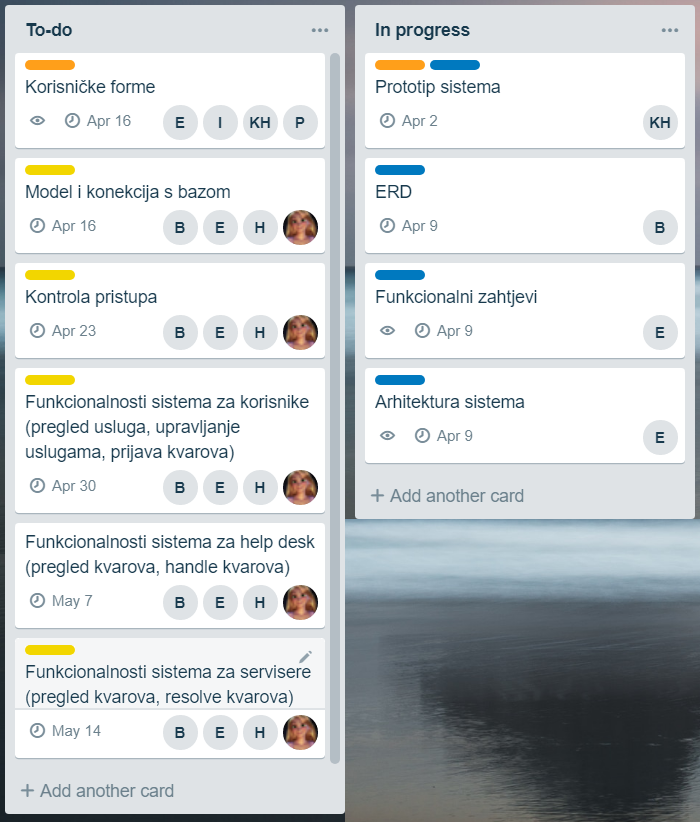
\includegraphics[scale=0.6]{../res/Trello/trello1.PNG}
\caption{\textit{Trello board} projekta, zadaci koji se trebaju izvršiti i koji se trenutno izvršavaju}
\label{trello1}
\end{figure}

\begin{figure}[H]
\center
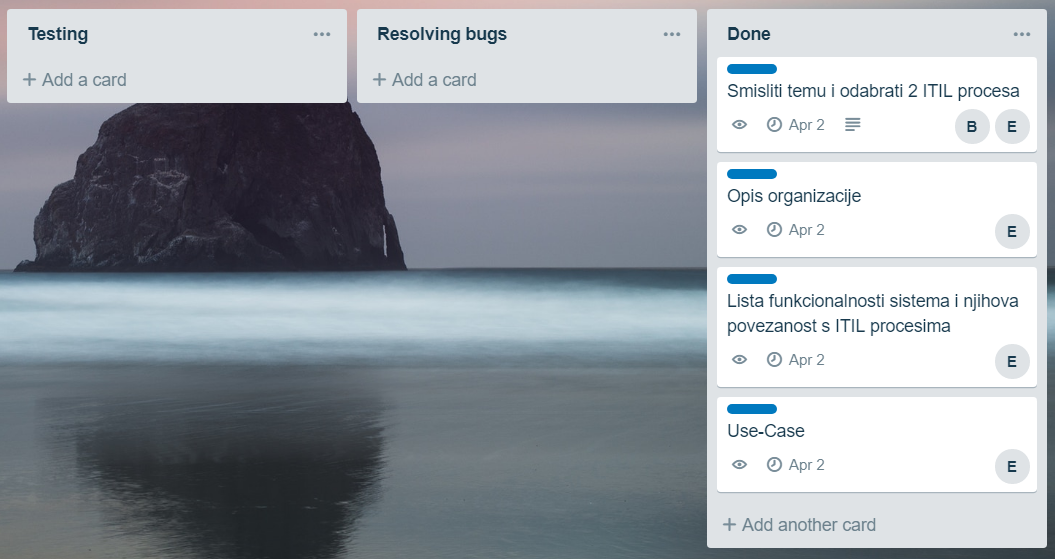
\includegraphics[scale=0.6]{../res/Trello/trello2.PNG}
\caption{\textit{Trello board} projekta, zadaci koji su završeni te dijelovi sistema koji se testiraju ili popravljaju}
\label{trello2}
\end{figure}

Prvi sprint razvoja aplikacije podrazumijevao je postojanje dva odvojena tima za razvoj. Timovi koji su razvijali \textit{backend} i \textit{frontend} dijelove aplikacije radili su odvojeno, budući da je konfigurisanje sistema, kreiranje CRUD operacija i ruta, kao i kreiranje početnih formi bilo nezavisno, te se na taj način sam proces završio brže i jednostavnije. Za dokumentaciju je bila zadužena jedna osoba, čije je zaduženje bilo koordinisanje timova i kreiranje pomoćne dokumentacije za razvoj. Prvi sprint prikazan je na slici \ref{trello3}, odakle je vidljivo da su zadaci timova bili potpuno različiti i nezavisni jedni od drugih.

\begin{figure}[H]
\center
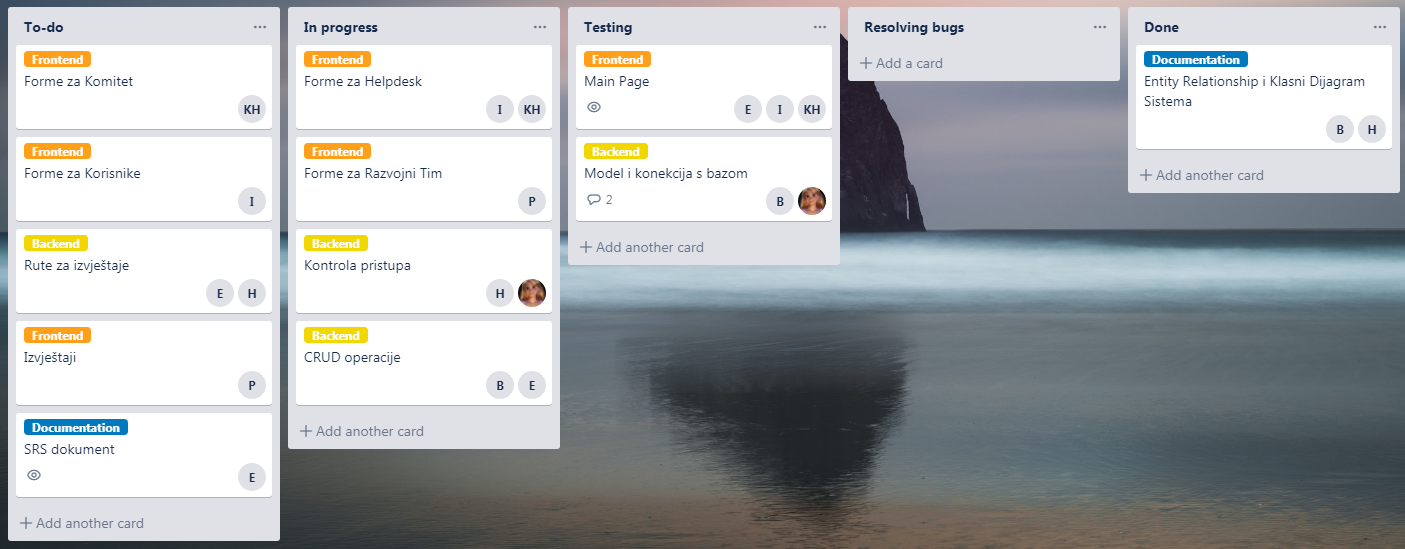
\includegraphics[scale=0.4]{../res/Trello/trello3.PNG}
\caption{Prvi sprint projekta}
\label{trello3}
\end{figure}

Drugi sprint razvoja aplikacije podrazumijevao je povezivanje dva dijela projekta koji su prethodno razvijeni. U okviru ovog sprinta \textit{frontend} tim izvršio je povezivanje na prethodno kreirane servise \textit{backend} tima, dok je \textit{backend} tim kreirao dodatne rute neophodne za prikaz izvještaja sistema. U ovom sprintu kreirana je formalna dokumentacija sistema koja opisuje funkcionalne i nefunkcionalne zahtjeve, prethodno kreiranu arhitekturu i korištene tehnologije, kao i sve ostale dijelove od kojih se ovaj dokument sastoji. Drugi sprint prikazan je na slici \ref{trello4}.

\begin{figure}[H]
\center
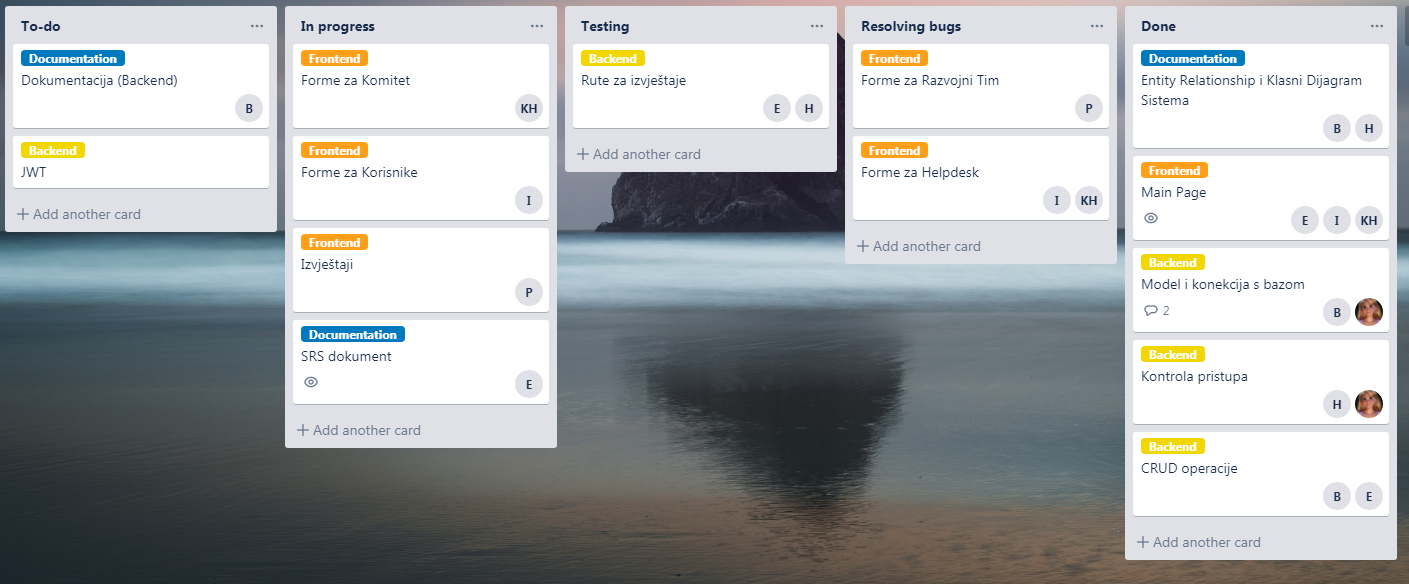
\includegraphics[scale=0.4]{../res/Trello/trello4.PNG}
\caption{Drugi sprint projekta}
\label{trello4}
\end{figure}

\newpage

\subsection{Prototip sistema}

\quad Na Slici \ref{pt1} prikazan je osnovni izgled ekrana aplikacije, koja ima korisnički interfejs kreiran poštujući pravila dobrog  dizajna.

\begin{figure}[H]
\center
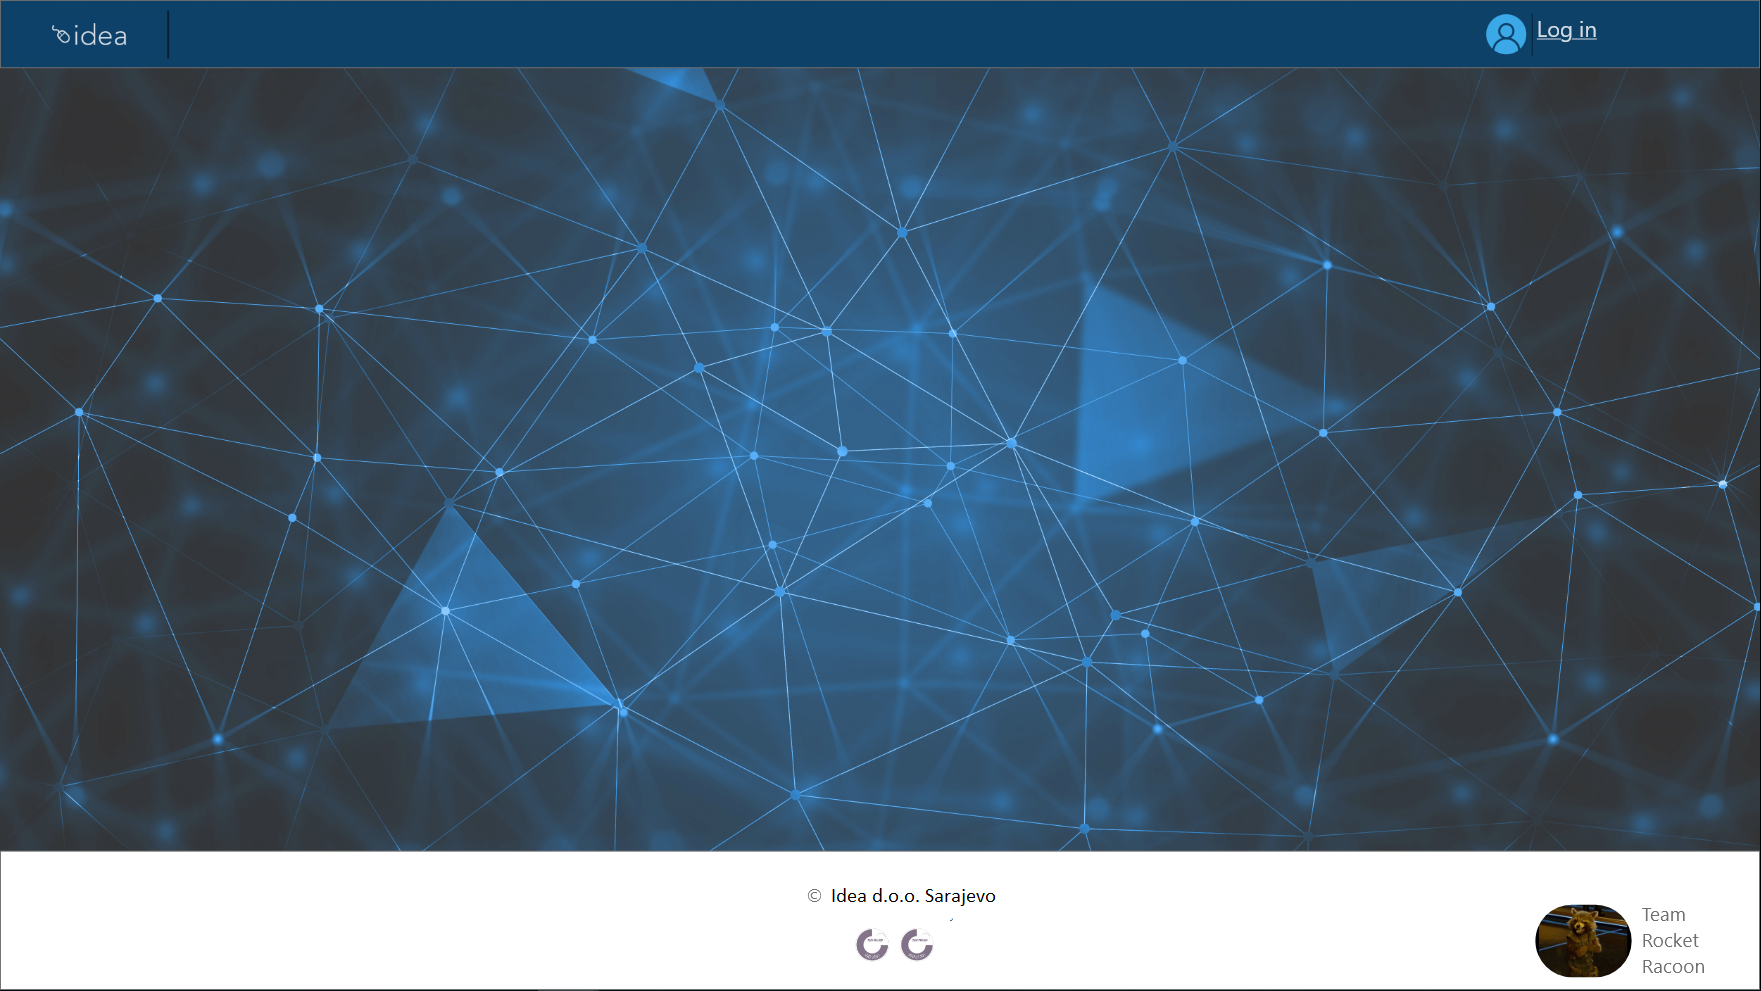
\includegraphics[scale=0.4]{../res/Prototype/Main.PNG}
\caption{Osnovni izgled ekrana aplikacije}
\label{pt1}
\end{figure}

Na Slici \ref{pt2} prikazan je izgled interfejsa za unos korisničkih podataka, nakon čega se omogućava pristup aplikaciji za različite vrste korisnika.

\begin{figure}[H]
\center
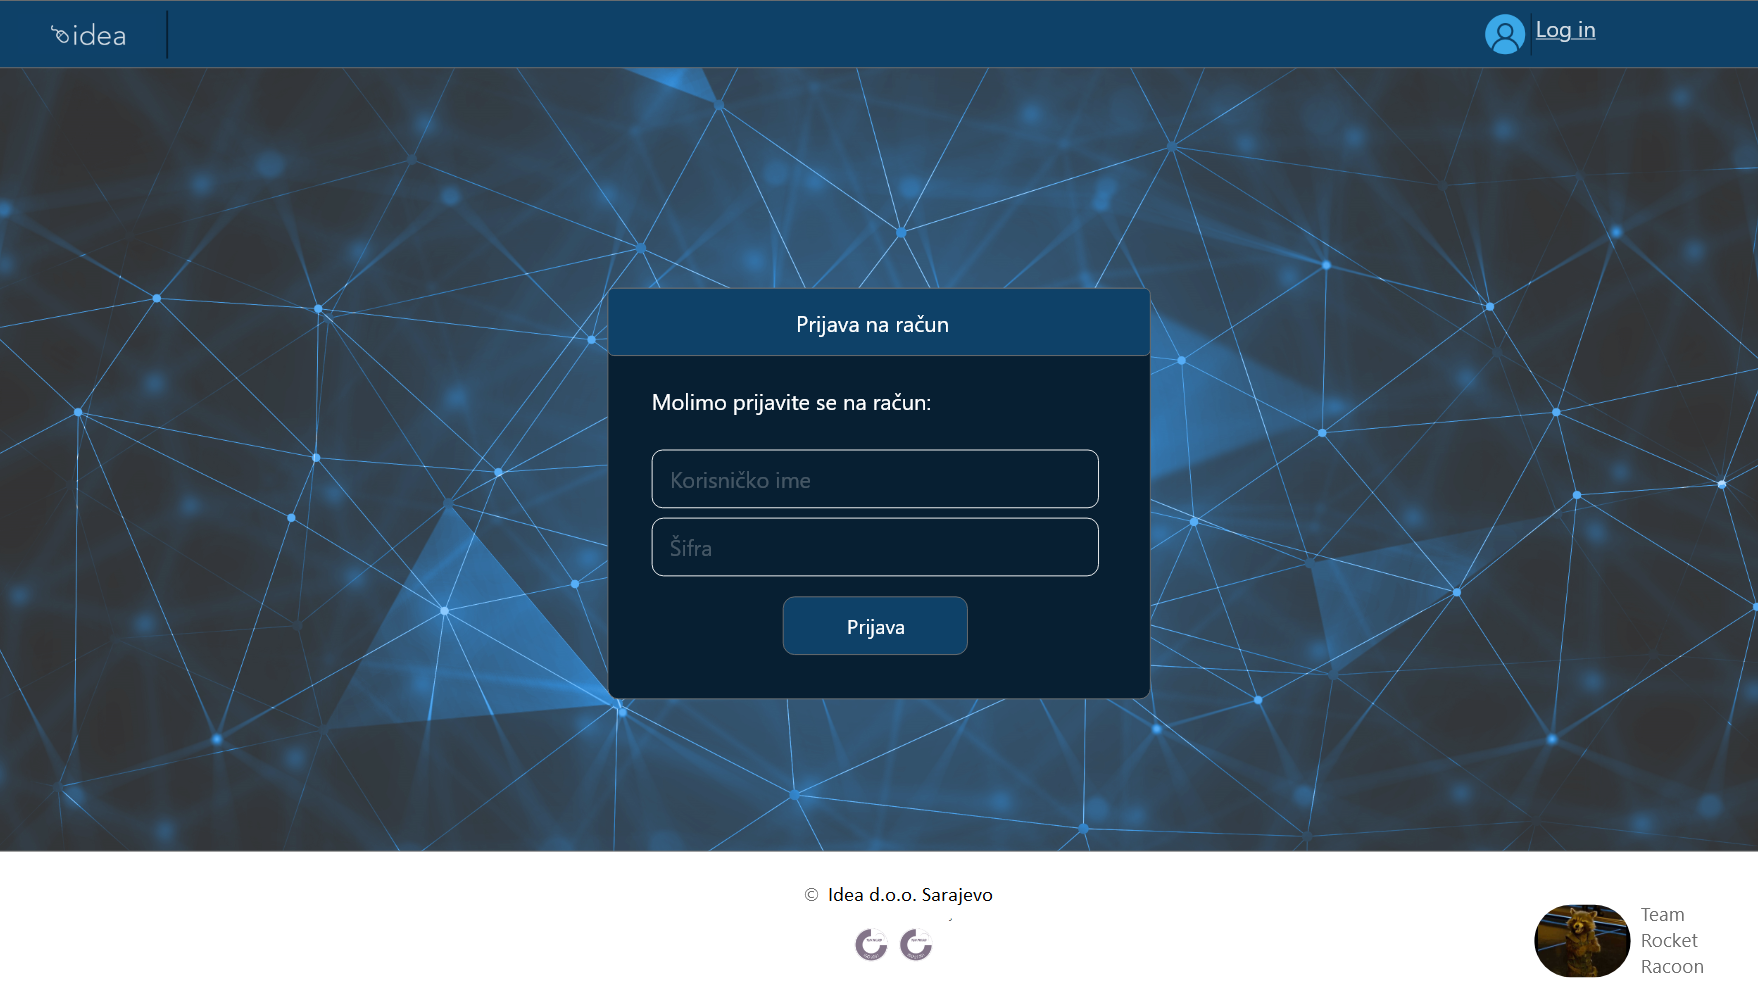
\includegraphics[scale=0.4]{../res/Prototype/LogIn.PNG}
\caption{Izgled interfejsa za unos korisničkih podataka}
\label{pt2}
\end{figure}

\newpage

Na Slici \ref{pt3} prikazan je izgled ekrana za pregled svih zahtjeva za promjenama, koje može vršiti tim za upravljanje promjenama. Nakon pregleda promjene, vrši se njena analiza i \textit{upload}-uje se PSO dokument, te se pritiskom na dugme \textbf{Prihvati} promjena automatski šalje komitetu za promjene. Alternativno, promjena se može odmah odbiti.

\begin{figure}[H]
\center
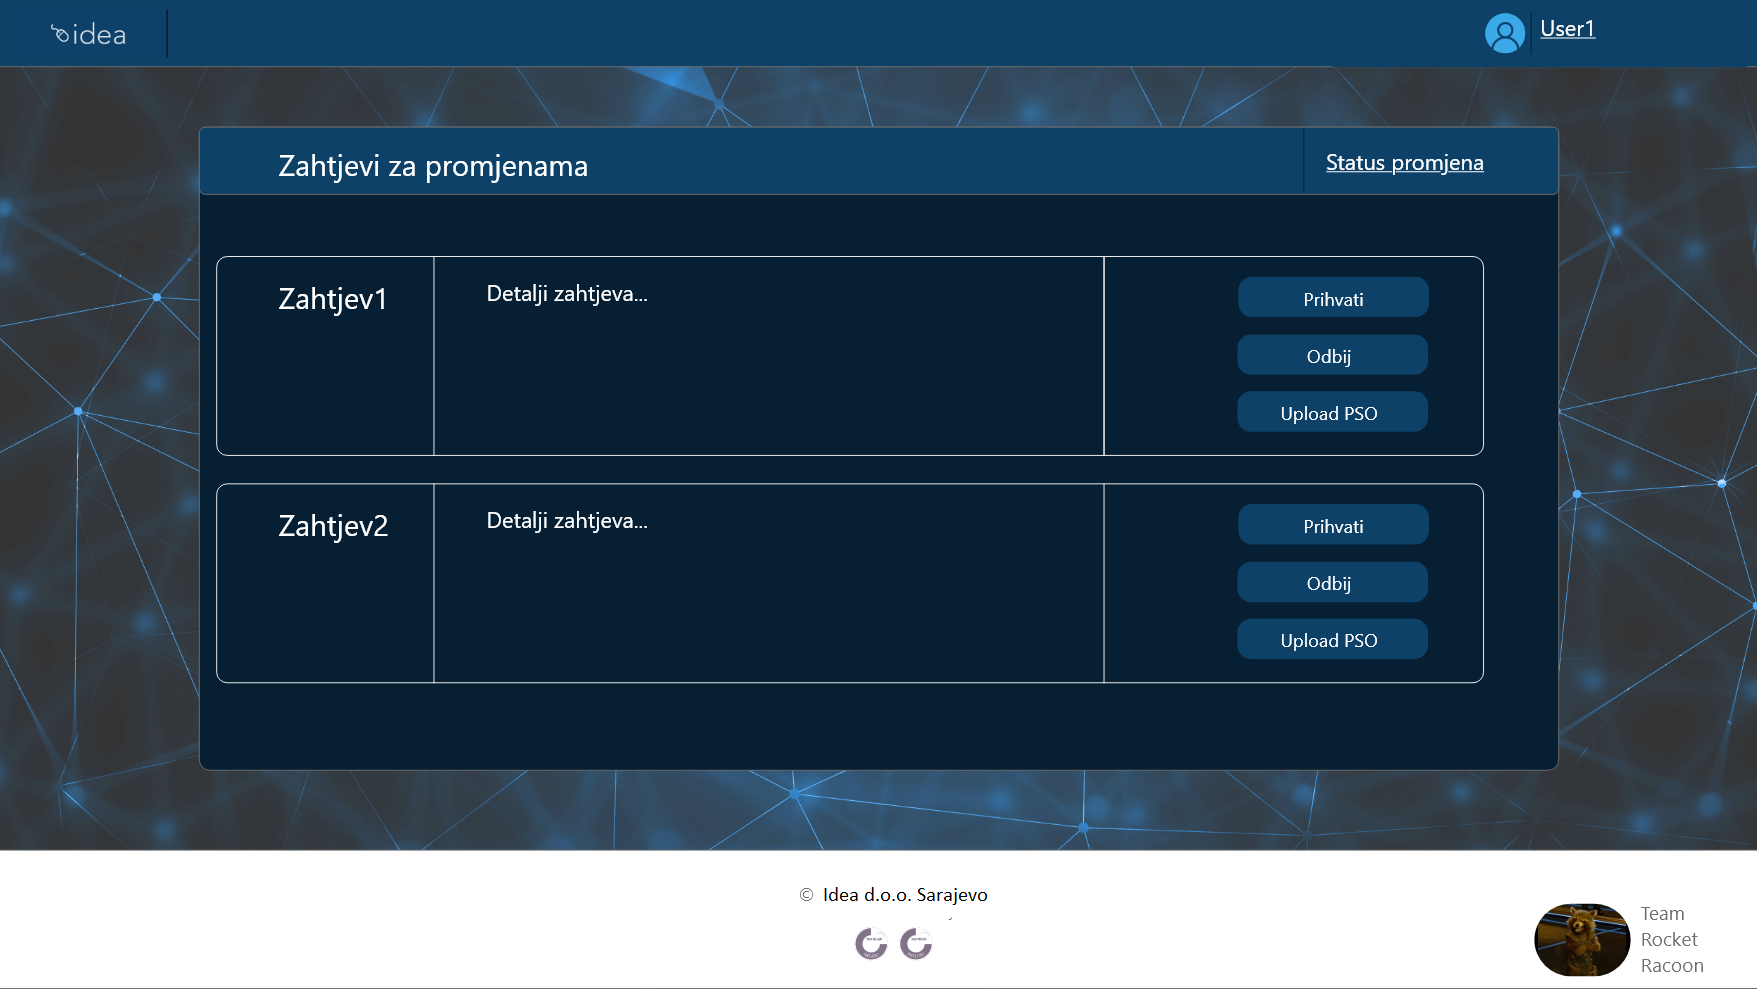
\includegraphics[scale=0.4]{../res/Prototype/Zahtjev-promjene.PNG}
\caption{Izgled interfejsa za pregled i procesiranje promjena}
\label{pt3}
\end{figure}

Na Slici \ref{pt4} prikazan je izgled ekrana za pregled svih odobrenih promjena, koje može vršiti tim za upravljanje promjenama. Promjene se mogu poslati razvojnom timu, te se vršiti njihov kontinualni nadzor i otkazivanje, ukoliko se pokaže da je promjenu nemoguće, vrlo teško ili neisplativo ugraditi u sistem.

\begin{figure}[H]
\center
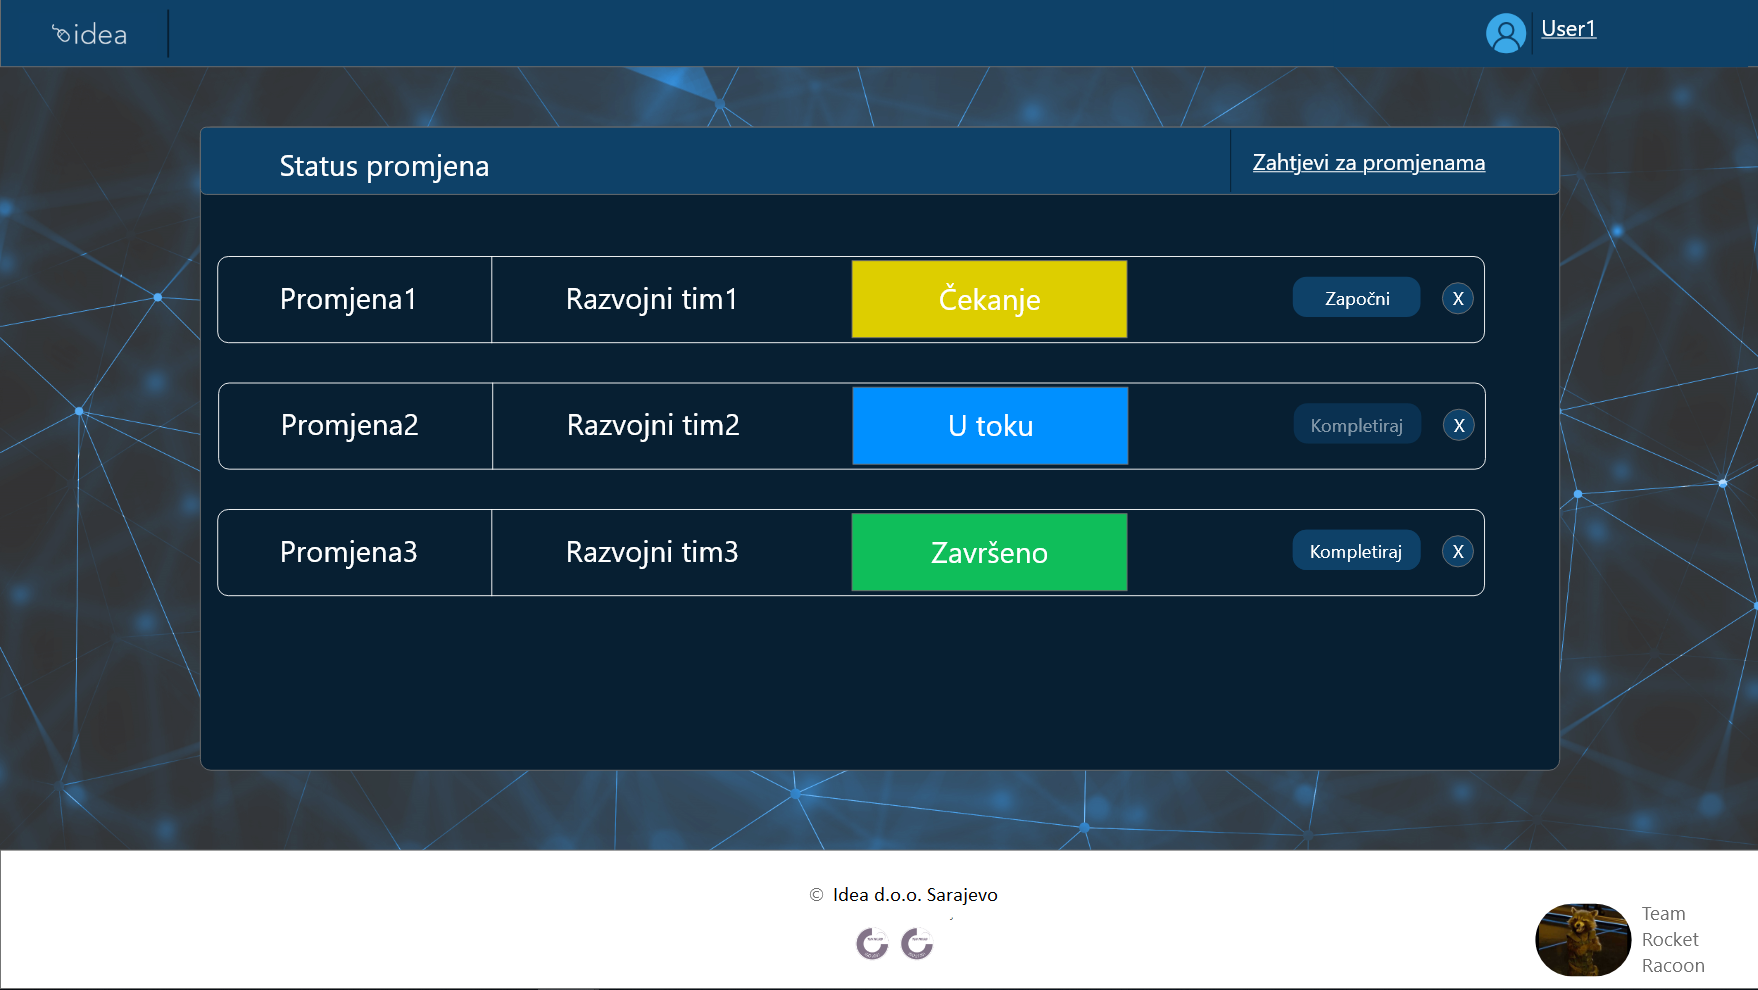
\includegraphics[scale=0.4]{../res/Prototype/Status-promjene.PNG}
\caption{Izgled interfejsa za pregled statusa odobrenih promjena}
\label{pt4}
\end{figure}

\newpage

Na Slici \ref{pt5} prikazan je izgled ekrana za prijavu greške od strane korisnika sistema koji se održava. Nakon unosa neophodnih informacija, greške se evidentiraju u sistemu kao događaji koje zatim pregleda tim za upravljanje promjenama te na koje adekvatno reaguje.

\begin{figure}[H]
\center
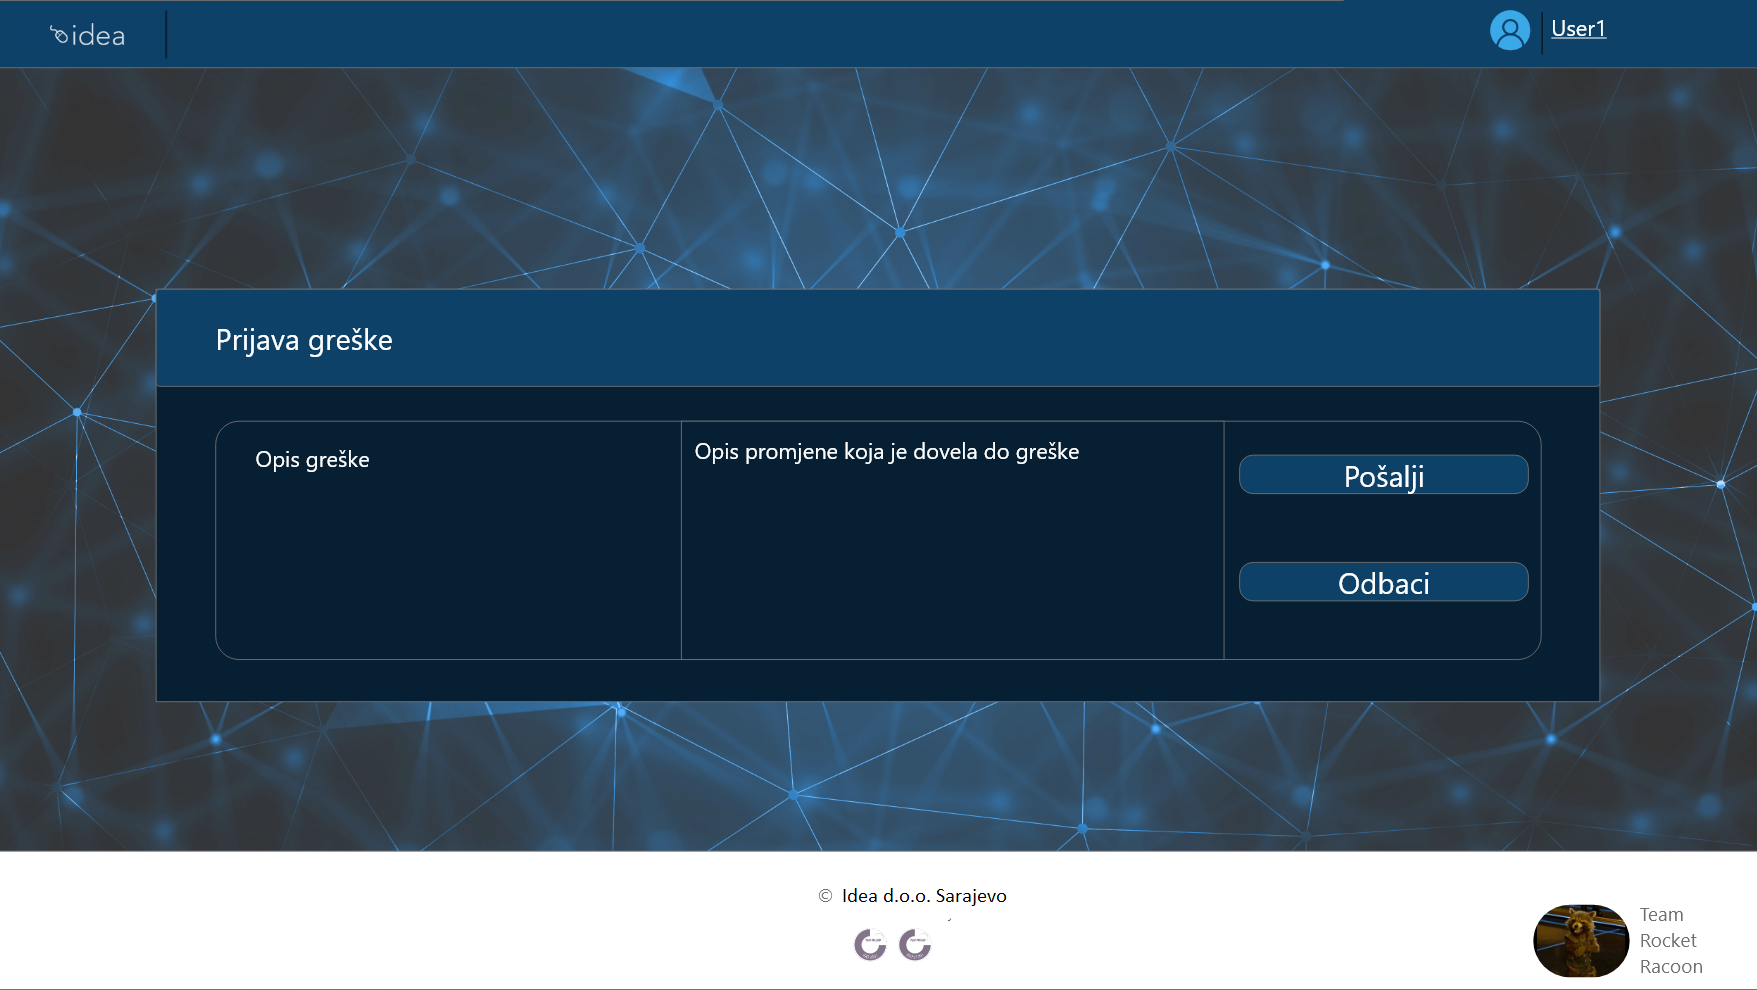
\includegraphics[scale=0.4]{../res/Prototype/Greske.PNG}
\caption{Izgled interfejsa za prijavu greške u sistemu}
\label{pt5}
\end{figure}

Na Slici \ref{pt6} prikazan je izgled ekrana za prijavu \textit{bug}-a od strane razvojnog tima. Nakon unosa neophodnih informacija, \textit{bug}-ovi se evidentiraju u sistemu kao događaji koje zatim pregleda tim za upravljanje promjenama te na koje adekvatno reaguje.

\begin{figure}[H]
\center
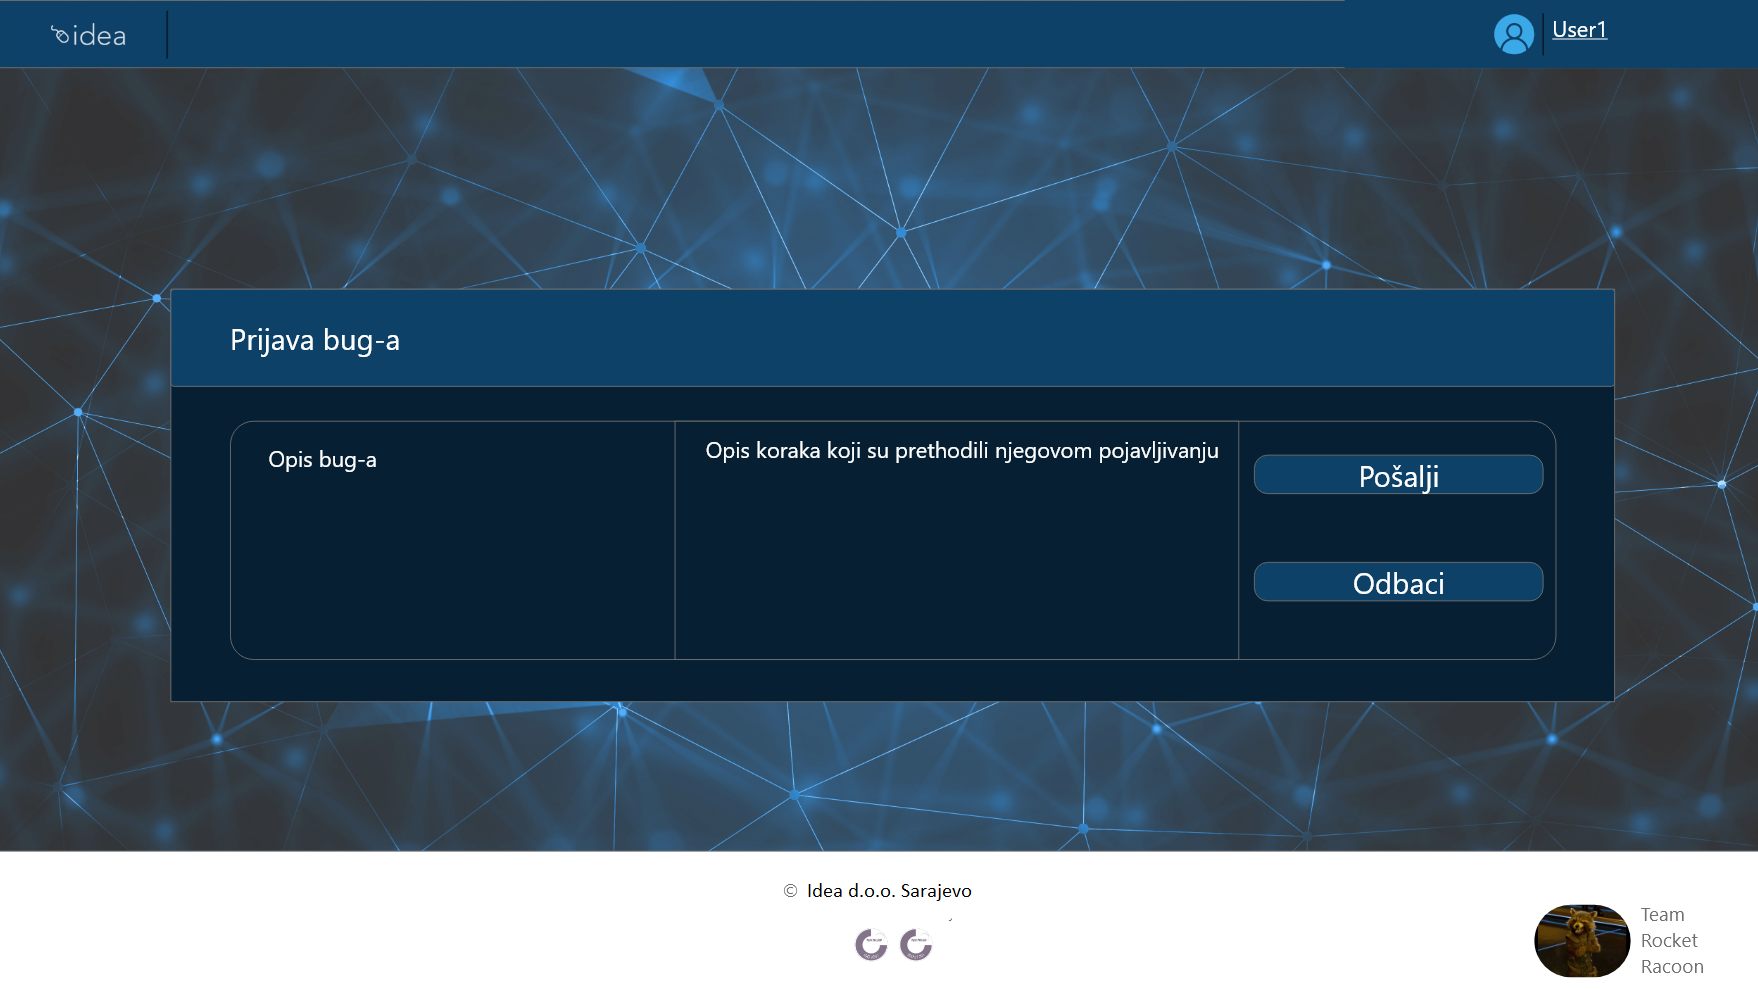
\includegraphics[scale=0.4]{../res/Prototype/Bugovi.PNG}
\caption{Izgled interfejsa za prijavu \textit{bug}-a u sistemu}
\label{pt6}
\end{figure}

\section{Funkcionalni zahtjevi}

\subsection{FZ 1. Prijava na sistem}

\subsubsection{Uvod}

Budući da nije omogućeno javno korištenje sistema, neophodno je izvršiti autorizaciju prije nego se korisniku dozvoli pristup. Osim toga, različite vrste korisnika imaju različite uloge u sistemu, te je potrebno izvršiti provjeru koju ulogu određeni korisnik ima, na osnovu čega se odobrava pristup samo određenim dijelovima sistema.

\subsubsection{Preduslovi}

Nema preduslova za ovaj funkcionalni zahtjev, budući da je svim korisnicima omogućena prijava na sistem.

\subsubsection{Ulazi}

Ulazi u proces prijave na sistem su korisnički podaci korisnika, koji se sastoje od \textit{korisničkog imena} i \textit {šifre}.

\subsubsection{Obrada}

Nakon što korisnik sistema unese svoje podatke, vrši se njihova usporedba s podacima iz baze podataka. Radi sigurnosti, u bazi se šifre čuvaju kao \textit{hash}-irane, te se pri provjeri validnosti podataka vrši \textit{hash}-iranje unesene šifre i usporedba s dobavljenim podacima iz baze. Ukoliko se pronađe poklapanje korisničkog imena i šifre, sistem preuzima podatke o ulozi korisnika u sistemu, te ovisno o ulozi korisnika preusmjerava na određenu početnu formu.

Cijeli proces prikazan je na Slici \ref{act1} u vidu dijagrama aktivnosti.

\begin{figure}[H]
\center
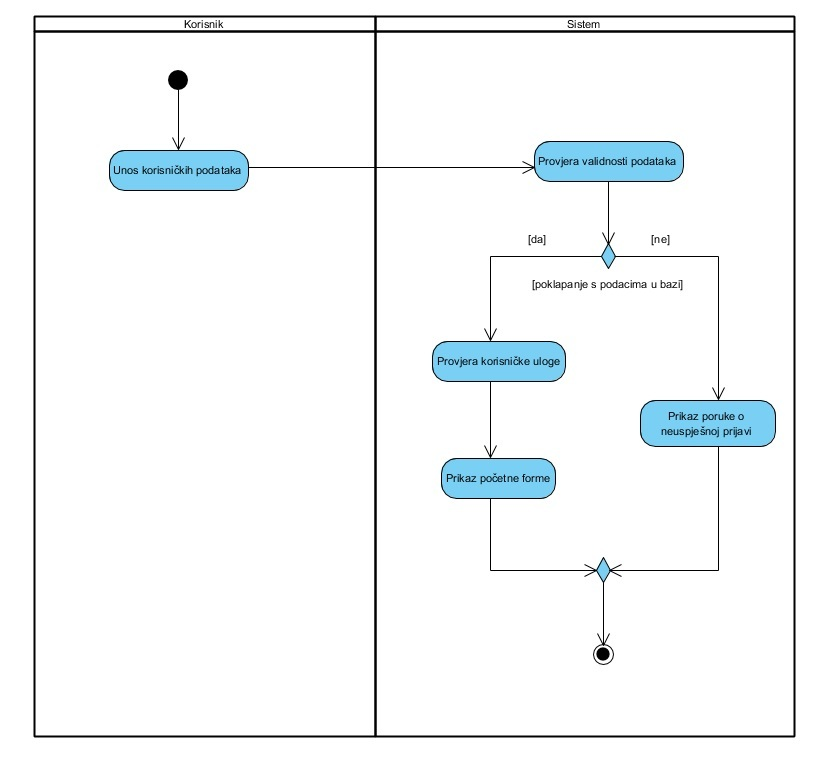
\includegraphics[scale=0.5]{../res/Activity/activity1.JPG}
\caption{Proces prijave na sistem}
\label{act1}
\end{figure}

\subsubsection{Izlazi}

Postoje dva moguća izlaza iz sistema - u slučaju unosa ispravnih korisničkih podataka, korisniku se omogućava pristup sistemu i preusmjerava se na odgovarajuću početnu formu, dok se u suprotnom slučaju prikazuje poruka o neispravnom unosu.

\subsubsection{Prioritet realizacije}

Prioritet realizacije ovog funkcionalnog zahtjeva je visok, budući da je vrlo važno omogućiti svim korisnicima prijavu na svoje korisničke račune.

\newpage

\subsection{FZ 2. Odjava sa sistema}

\subsubsection{Uvod}

Nakon što korisnik završi s korištenjem sistema, može se odjaviti s istog. Svim korisnicima sistema omogućeno je vršenje odjave sa sistema na isti način. Zbog sigurnosti, nakon vršenja odjave sa sistema završava se korisnička sesija, te se onemogućava pristup sistemu dok se ponovo ne unesu ispravni korisnički podaci.

\subsubsection{Preduslovi}

Da bi se korisnik mogao odjaviti, prvo mora biti prijavljen na svoj korisnički račun.

\subsubsection{Ulazi}

Ulaz u sistem predstavlja pritisak na dugme za odjavu.

\subsubsection{Obrada}

Nakon što korisnik pritisne na dugme za odjavu, sistem vrši završavanje korisničke sesije, odnosno onemogućava datom korisniku dalje korištenje sistema. Nakon toga, korisnik se preusmjerava na formu za prijavu.

Cijeli proces prikazan je na Slici \ref{act2} u vidu dijagrama aktivnosti.

\begin{figure}[H]
\center
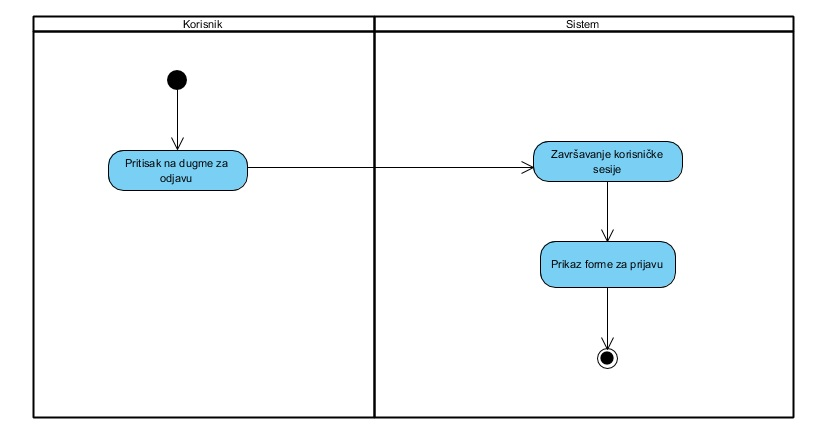
\includegraphics[scale=0.5]{../res/Activity/activity2.JPG}
\caption{Proces odjave sa sistema}
\label{act2}
\end{figure}

\subsubsection{Izlazi}

Izlaz iz sistema je preusmjeravanje na formu za prijavu.

\subsubsection{Prioritet realizacije}

Prioritet realizacije ovog zahtjeva je visok, jer neuspješna odjava sa sistema omogućava zlonamjernim korisnicima zloupotrebu aktivne sesije.

\newpage

\subsection{FZ 3. Slanje zahtjeva za promjenom}

\subsubsection{Uvod}

Korisnici aplikacija koje firma Idea razvija mogu poslati zahtjeve za promjenama. Kako bi to izvršili, potrebno je unijeti odgovarajuće podatke o zahtjevu te poslati isti kako bi ga nakon toga nadležna lica mogla obraditi.

\subsubsection{Preduslovi}

Slanje zahtjeva za promjenom omogućeno je samo korisnicima koji su prijavljeni kao korisnici softvera koje firma Idea razvija.

\subsubsection{Ulazi}

Ulaz u sistem predstavlja sam zahtjev za promjenom, koji je opisan putem sljedećih podataka:

\begin{itemize}
\item Opis zahtjeva;
\item Vrsta zahtjeva (jedna od predefinisanih vrijednosti iz liste: promjena sistema, promjena usluge, ostalo).
\end{itemize}

\subsubsection{Obrada}

Nakon što se korisnik softvera prijavi na sistem, treba unijeti podatke o zahtjevu i odabrati opciju za slanje. U svakom trenutku prije slanja omogućeno je brisanje zahtjeva.

Cijeli proces prikazan je na Slici \ref{act3} u vidu dijagrama aktivnosti.

\begin{figure}[H]
\center
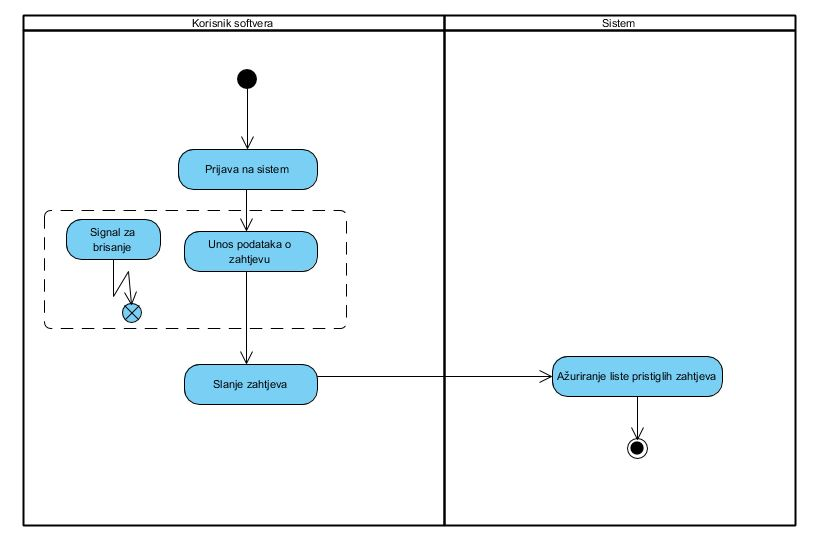
\includegraphics[scale=0.5]{../res/Activity/activity3.JPG}
\caption{Proces slanja zahtjeva za promjenom}
\label{act3}
\end{figure}

\subsubsection{Izlazi}

Izlaz iz sistema predstavlja poruka o uspješnom slanju zahtjeva za promjenom.

\subsubsection{Prioritet realizacije}

Prioritet realizacije ovog funkcionalnog zahtjeva je nizak, jer je slanje zahtjeva za promjenom proces koji se može odložiti u slučaju nedostupnosti sistema.

\newpage

\subsection{FZ 4. Prijava grešaka}

\subsubsection{Uvod}

Korisnici sistema kojima je omogućeno prijavljivanje grešaka su korisnici softvera i članovi tima za razvoj i produkciju. Korisnici sistema mogu prijavljivati greške pri korištenju softvera, dok članovi razvojnog tima mogu prijaviti \textit{bug}-ove (funkcionalnosti koje ne rade ispravno te koje je potrebno popraviti) i nemogućnost implementacije nekog od zahtjeva za promjene. U svim slučajevima, prijave se prosljeđuju \textit{helpdesk}-u koji vrši njihovo raspoređivanje.

\subsubsection{Preduslovi}

Prijava grešaka omogućena je korisnicima softvera koje firma Idea razvija i članovima razvojnog tima firme.

\subsubsection{Ulazi}

Ulaz u sistem predstavlja prijava greške, koja je opisana putem sljedećih podataka:

\begin{itemize}
\item Opis greške:
\item Vrsta greške (u slučaju razvojnog tima, moguće je grešku klasificirati kao \textit{bug}, sistemsku grešku ili ostalo).
\end{itemize}

\subsubsection{Obrada}

Nakon što se korisnik prijavi na sistem, treba unijeti podatke o grešci i odabrati opciju za slanje. U svakom trenutku prije slanja omogućeno je brisanje prijave.

Cijeli proces prikazan je na Slici \ref{act4} u vidu dijagrama aktivnosti.

\begin{figure}[H]
\center
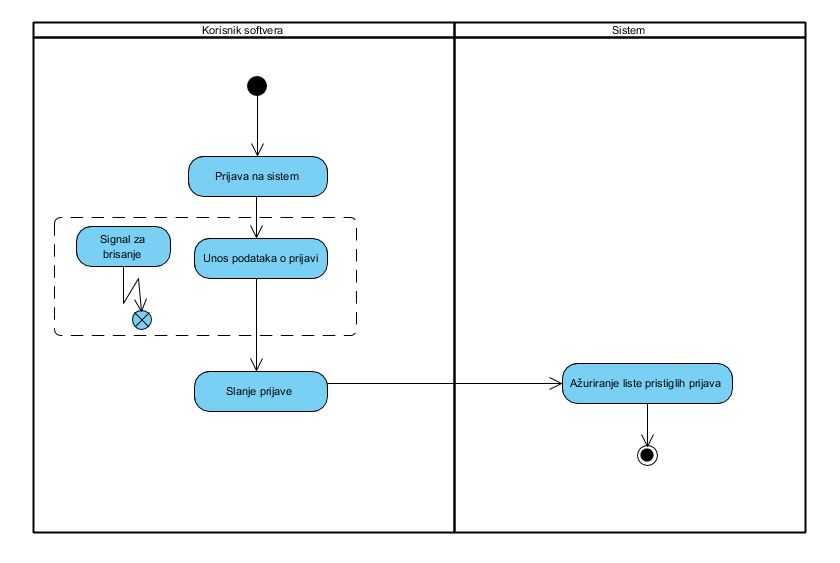
\includegraphics[scale=0.5]{../res/Activity/activity4.JPG}
\caption{Proces slanja prijave greške}
\label{act4}
\end{figure}

\subsubsection{Izlazi}

Izlaz iz sistema predstavlja poruka o uspješnom slanju prijave greške.

\subsubsection{Prioritet realizacije}

Prioritet realizacije ovog funkcionalnog zahtjeva je srednji, jer je važno ispraviti greške što prije kako bi korisnici mogli nesmetano koristiti aplikacije firme Idea.

\newpage

\subsection{FZ 5. Pregled svih prijava}

\subsubsection{Uvod}

Članovi razvojnog tima mogu pregledati listu svih pristiglih prijava koje su im dodijeljene od strane \textit{helpdesk}-a. Korisnici softvera mogu pregledati listu svih prijava koje su poslali. \textit{Helpdesk} može pregledati listu svih prijava za sve korisnike i sve razvojne timove. U okviru liste koju mogu pregledati nalaze se greške u sistemu (koje su prijavili korisnici ili članovi razvojnog tima), kao i zahtjevi koje je potrebno implementirati. Nakon uspješne implementacije ili popravljanja grešaka, omogućeno je njihovo arhiviranje.

\subsubsection{Preduslovi}

Pregled svih prijava omogućen je članovima razvojnog tima, budući da je lista prijava prilagođena aktivnostima koje razvojni tim vrši (implementacija novih zahtjeva i ispravljanje grešaka). Da bi se prijava prikazala u listi, potrebno je da je \textit{helpdesk} prvo rasporedi datom razvojnom timu. Pregled svih prijava u sistemu omogućen je i \textit{helpdesk}-u (bez filtriranja), budući da oni u svakom trenutku trebaju imati uvid u sve što se dešava u sistemu. Pregled svih prijava koje je korisnik prijavio omogućene su korisniku softvera.

\subsubsection{Ulazi}

Nema ulaza u sistem - nakon uspješne prijave, svim članovima razvojnog tima omogućen je isti pregled svih prijava.

\subsubsection{Obrada}

Obrada zahtjeva sastoji se u dobavljanju svih podataka o prijavama te vršenje njihovog filtriranja ovisno o tome kojoj vrsti korisnika ili kojem razvojnom timu korisnik pripada.

Cijeli proces prikazan je na Slici \ref{act5} u vidu dijagrama aktivnosti.

\begin{figure}[H]
\center
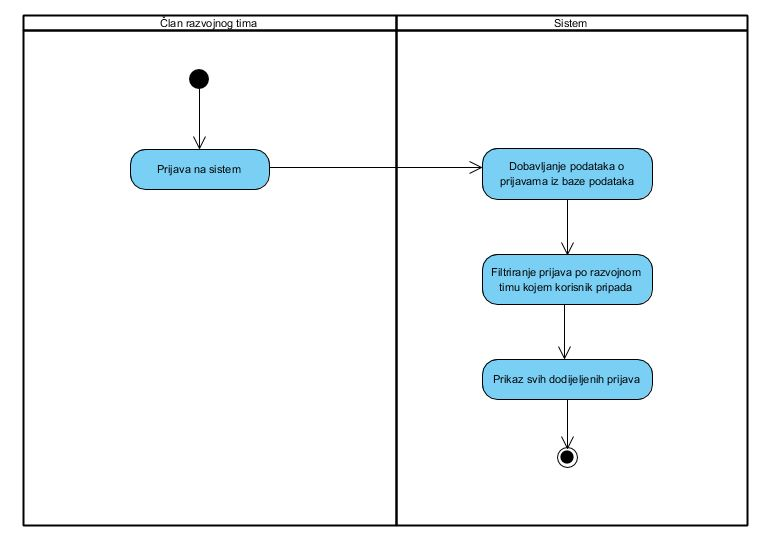
\includegraphics[scale=0.5]{../res/Activity/activity5.JPG}
\caption{Proces pregleda svih prijava}
\label{act5}
\end{figure}

\subsubsection{Izlazi}

Izlaz iz sistema predstavlja prikaz liste svih dodijeljenih prijava sa svim pripadajućim podacima.

\subsubsection{Prioritet realizacije}

Prioritet realizacije ovog funkcionalnog zahtjeva je srednji, budući da je neophodno što prije prikazati prijave timu za produkciju kako bi se greške mogle ispraviti.

\newpage

\subsection{FZ 6. Arhiviranje prijava}

\subsubsection{Uvod}

Članovi razvojnog tima vrše popravljanje prijavljenih grešaka te implementiranje dodijeljenih zahtjeva za promjenama. Nakon uspješnog vršenja implementacije, vrše arhiviranje istih kako bi se uklonile s liste aktivnih prijava. Arhiviranje je omogućeno i \textit{helpdesk}-u.

\subsubsection{Preduslovi}

Arhiviranje prijava omogućeno je isključivo članovima tima za razvoj i \textit{helpdesk}-u. Da bi se prijava arhivirala, prvo se mora početi s njenom implementacijom (njen status mora biti \textit{U toku}).

\subsubsection{Ulazi}

Ulaz u sistem je pritisak na dugme za arhiviranje prijave.

\subsubsection{Obrada}

Nakon što autorizovani korisnik pritisne na dugme za arhiviranje, sistem vrši označavanje prijave arhiviranom te je uklanja iz liste aktivnih prijava.

Cijeli proces prikazan je na Slici \ref{act6} u vidu dijagrama aktivnosti.

\begin{figure}[H]
\center
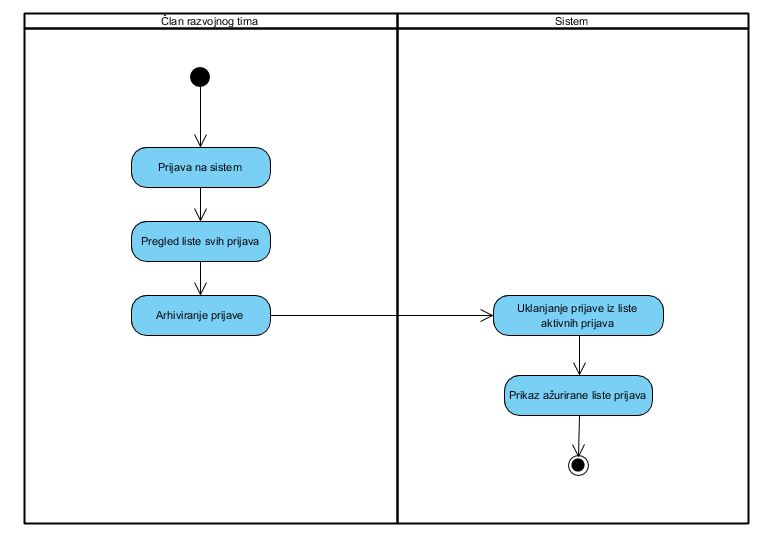
\includegraphics[scale=0.5]{../res/Activity/activity6.JPG}
\caption{Proces arhiviranja prijave}
\label{act6}
\end{figure}

\subsubsection{Izlazi}

Izlaz iz sistema je ažurirana lista prijava, koja ne sadrži arhiviranu prijavu.

\subsubsection{Prioritet realizacije}

Prioritet realizacije ovog funkcionalnog zahtjeva je nizak, budući da arhiviranje implementirane prijave nije prioritetna akcija.

\newpage

\subsection{FZ 7. Pregled svih pristiglih zahtjeva}

\subsubsection{Uvod}

Nakon što korisnik pošalje zahtjev za promjenom i \textit{helpdesk} napravi studiju izvodljivosti i odobri zahtjev, on se šalje komitetu za promjene na pregled i konačno odlučivanje. Iz tog razloga komitet za promjene treba imati omogućen pregled svih pristiglih zahtjeva o kojima je potrebno odlučivati. Pregled svih zahtjeva omogućen je i \textit{helpdesk}-u, koji u svakom trenutku treba imati uvid u sve dijelove sistema. Pregled zahtjeva koje je korisnik poslao omogućeno je tom korisniku.

\subsubsection{Preduslovi}

Pregled svih pristiglih zahtjeva omogućen je komitetu za promjene, korisnicima softvera i \textit{helpdesk}-u. Da bi se zahtjev prikazao u listi komiteta za promjene, \textit{helpdesk} ga prvo mora odobriti i priložiti PSO dokument za komitet.

\subsubsection{Ulazi}

Nema ulaza u sistem - nakon uspješne prijave, svim članovima komiteta za promjene omogućen je isti pregled svih pristiglih zahtjeva.

\subsubsection{Obrada}

Obrada zahtjeva sastoji se u dobavljanju svih podataka o zahtjevima koje je \textit{helpdesk} odobrio.

Cijeli proces prikazan je na Slici \ref{act7} u vidu dijagrama aktivnosti.

\begin{figure}[H]
\center
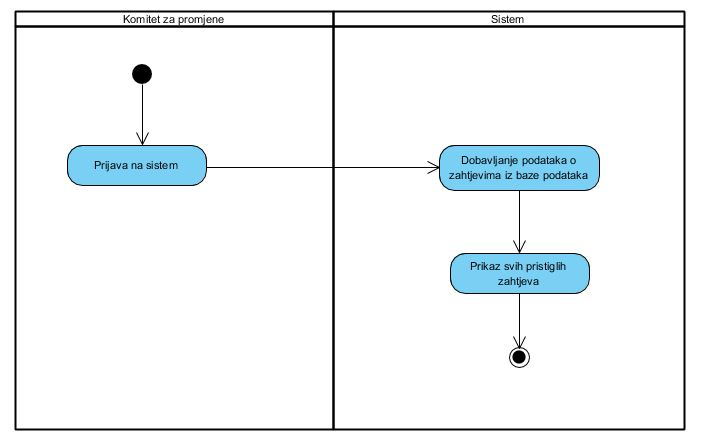
\includegraphics[scale=0.5]{../res/Activity/activity7.JPG}
\caption{Proces pregleda svih pristiglih zahtjeva}
\label{act7}
\end{figure}

\subsubsection{Izlazi}

Izlaz iz sistema predstavlja prikaz liste svih dodijeljenih prijava sa svim pripadajućim podacima.

\subsubsection{Prioritet realizacije}

Prioritet realizacije ovog funkcionalnog zahtjeva je srednji, budući da je potrebno što prije pregledati novopristigle zahtjeve, no ukoliko bi sistem bio nedostupan, ta akcija bi mogla biti odložena.

\newpage

\subsection{FZ 8. Odlučivanje po zahtjevu}

\subsubsection{Uvod}

Nakon pregleda svih informacija o pristiglom zahtjevu (uključujući detalje zahtjeva i PSO dokument), komitet za promjene donosi konačnu odluku. Ovisno o tome kakva je konačna odluka, zahtjev se ili arhivira, ili vraća u listu za \textit{helpdesk} kako bi se moglo početi s njegovom implementacijom.

\subsubsection{Preduslovi}

Odlučivanje po zahtjevima omogućeno je samo komitetu za promjene. Da bi se odlučivalo o nekom zahtjevu, on prvo mora biti u listi pristiglih zahtjeva (mora biti odobren od strane \textit{helpdesk}-a).

\subsubsection{Ulazi}

Ulaz u sistem predstavlja konačna odluka komiteta - odobravanje ili odbijanje zahtjeva.

\subsubsection{Obrada}

Nakon unosa konačne odluke o zahtjevu (pritiska na dugme za odobravanje ili odbijanje zahtjeva), sistem vrši ažuriranje liste događaja \textit{helpdesk}-a ili arhiviranje zahtjeva.

Cijeli proces prikazan je na Slici \ref{act8} u vidu dijagrama aktivnosti.

\begin{figure}[H]
\center
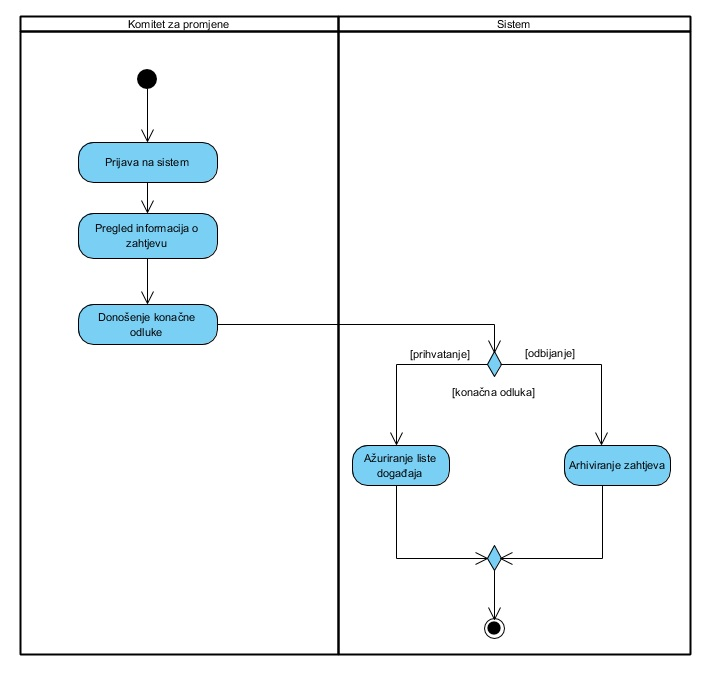
\includegraphics[scale=0.5]{../res/Activity/activity8.JPG}
\caption{Proces odlučivanja po zahtjevu}
\label{act8}
\end{figure}

\subsubsection{Izlazi}

Izlaza iz sistema nema - nakon što se odluči po zahtjevu, isti se uklanja iz liste pristiglih zahtjeva tako da član komiteta za promjene može postupati po drugim zahtjevima.

\subsubsection{Prioritet realizacije}

Prioritet realizacije ovog funkcionalnog zahtjeva je srednji, budući da je potrebno što prije poslati zahtjev na implementaciju (ukoliko se odobri), no to nije akcija s najvišim prioritetom.

\newpage

\subsection{FZ 9. Pregled svih događaja u sistemu}

\subsubsection{Uvod}

Članovi \textit{helpdesk}-a trebaju vršiti raspoređivanje zahtjeva i prijava odgovarajućim korisnicima sistema na dalju obradu. Iz tog razloga komitet za promjene treba imati omogućen pregled svih događaja (pristiglih zahtjeva i prijava) koje je potrebno raspoređivati.

\subsubsection{Preduslovi}

Pregled svih događaja u sistemu omogućen je samo \textit{helpdesk}-u.

\subsubsection{Ulazi}

Nema ulaza u sistem - nakon uspješne prijave, svim članovima \textit{helpdesk}-a omogućen je isti pregled svih događaja u sistemu.

\subsubsection{Obrada}

Obrada zahtjeva sastoji se u dobavljanju svih podataka o događajima (svi pristigli zahtjevi, odobreni zahtjevi te prijave korisnika i članova razvojnog tima).

Cijeli proces prikazan je na Slici \ref{act9} u vidu dijagrama aktivnosti.

\begin{figure}[H]
\center
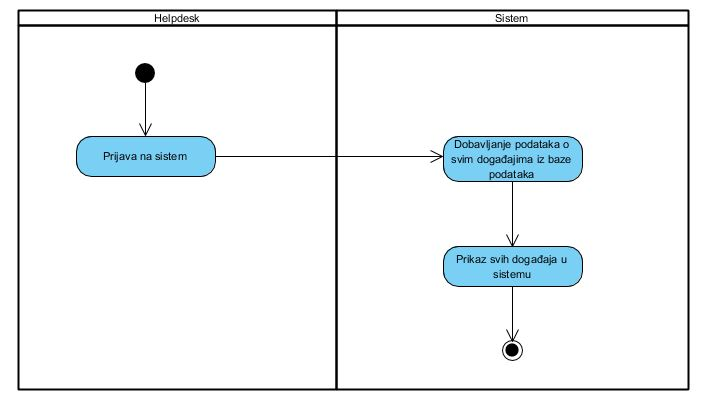
\includegraphics[scale=0.5]{../res/Activity/activity9.JPG}
\caption{Proces pregleda svih događaja u sistemu}
\label{act9}
\end{figure}

\subsubsection{Izlazi}

Izlaz iz sistema predstavlja prikaz liste svih događaja u sistemu sa svim pripadajućim podacima.

\subsubsection{Prioritet realizacije}

Prioritet realizacije ovog funkcionalnog zahtjeva je visok, jer \textit{helpdesk} mora moći nesmetano vršiti raspoređivanje događaja, a preduslov za to je mogućnost pregledanja svih događaja.

\newpage

\subsection{FZ 10. Slanje zahtjeva na konačno odlučivanje}

\subsubsection{Uvod}

Nakon što korisnik softvera pošalje zahtjev, on se prikazuje \textit{helpdesk}-u u listi svih događaja u sistemu. Nakon toga članovi \textit{helpdesk}-a vrše procjenu izvodljivosti koja se, zajedno sa svim ostalim relevantnim informacijama, nalazi u PSO dokumentu. Tada se zahtjev šalje komitetu za promjene na konačno odlučivanje.

\subsubsection{Preduslovi}

Slanje zahtjeva na konačno odlučivanje omogućeno je samo \textit{helpdesk}-u. Zahtjev prvo treba ispuniti uslove za odobravanje, odnosno studija izvodljivosti treba dati pozitivne rezultate.

\subsubsection{Ulazi}

Ulaz u sistem predstavlja PSO dokument, koji je neophodno priložiti uz zahtjev kako bi se isti poslao na konačno odlučivanje. PSO dokument prilaže se u obliku PDF dokumenta.

\subsubsection{Obrada}

Nakon uspješne prijave i odabira zahtjeva iz liste svih događaja u sistemu, član \textit{helpdesk}-a prilaže PSO dokument i vrši pritisak na dugme za slanje zahtjeva na konačno odlučivanje. Nakon toga se ažurira status zahtjeva u listi koju \textit{helpdesk} vidi, te se zahtjev dodaje u listu pristiglih zahtjeva o kojima komitet treba odlučivati.

Cijeli proces prikazan je na Slici \ref{act10} u vidu dijagrama aktivnosti.

\begin{figure}[H]
\center
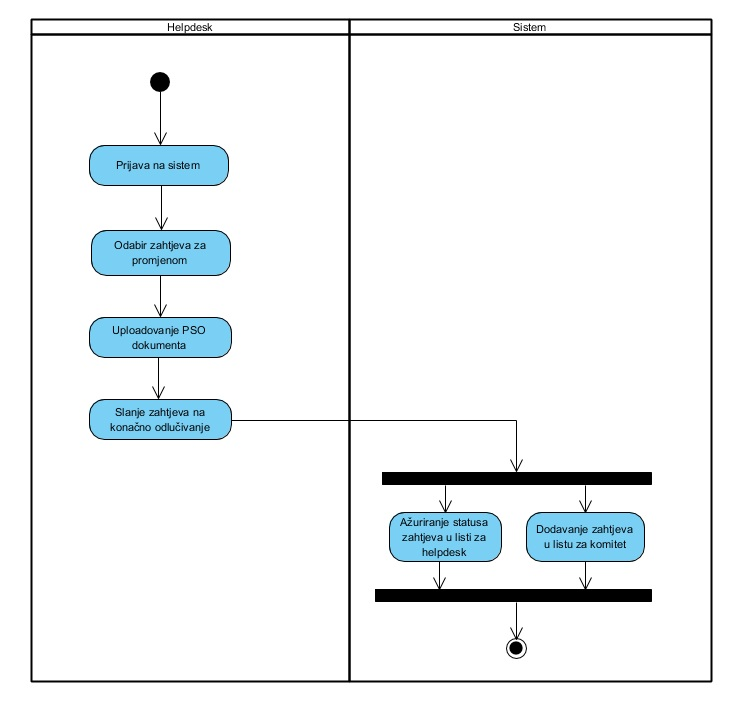
\includegraphics[scale=0.5]{../res/Activity/activity10.JPG}
\caption{Proces slanja zahtjeva na konačno odlučivanje}
\label{act10}
\end{figure}

\subsubsection{Izlazi}

Izlaz iz sistema predstavlja prikaz ažurirane liste svih događaja u sistemu, u kojoj poslani zahtjev ima promijenjen status.

\subsubsection{Prioritet realizacije}

Prioritet realizacije ovog funkcionalnog zahtjeva je nizak, budući da slanje zahtjeva na konačno odlučivanje nije hitno i može se odložiti u slučaju nedostupnosti sistema.

\newpage

\subsection{FZ 11. Raspoređivanje događaja}

\subsubsection{Uvod}

\textit{Helpdesk} predstavlja skup korisnika sistema koji mogu pregledati sve događaje u sistemu, i čija je dužnost njihovo raspoređivanje onim korisnicima sistema koji trebaju postupati po njima. Jedna od najvažnijih funkcionalnosti ovih korisnika je olakšavanje rada ostalim korisnicima, jer će svi vidjeti samo one događaje koji su za njih relevantni.

\subsubsection{Preduslovi}

Raspoređivanje događaja može vršiti samo \textit{helpdesk}.

\subsubsection{Ulazi}

Postoje sljedeći ulazi u sistem:

\begin{itemize}
\item Odabir vrste korisnika kojem se dati događaj treba dodijeliti:
\item Odabir prioriteta događaja;
\item Odabir statusa događaja.
\end{itemize}

\subsubsection{Obrada}

Nakon prijave na sistem, član \textit{helpdesk}-a odabire događaj koji je potrebno rasporediti. Nakon unosa neophodnih podataka i pritiska na dugme za raspoređivanje, prikazuje se ažurirana lista događaja na kojoj je prikazano kome je događaj dodijeljen i kakav je njegov status.

Cijeli proces prikazan je na Slici \ref{act11} u vidu dijagrama aktivnosti.

\begin{figure}[H]
\center
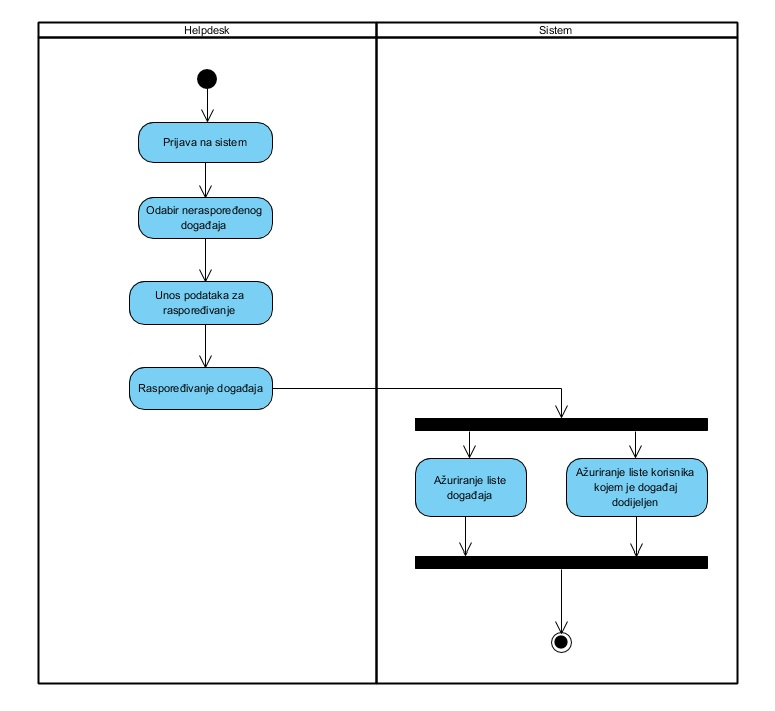
\includegraphics[scale=0.5]{../res/Activity/activity11.JPG}
\caption{Proces raspoređivanja događaja}
\label{act11}
\end{figure}

\subsubsection{Izlazi}

Izlaz iz sistema predstavlja prikaz ažurirane liste svih događaja u sistemu, u kojoj raspoređeni događaj ima promijenjen status.

\subsubsection{Prioritet realizacije}

Prioritet realizacije ovog funkcionalnog zahtjeva je visok, jer \textit{helpdesk} treba u svakom trenutku moći izvršiti raspoređivanje događaja (poput grešaka zbog kojih su aplikacije nedostupne korisnicima) adekvatnim korisnicima sistema.

\newpage

\subsection{FZ 12. Pregled izvještaja}

\subsubsection{Uvod}

Članovi \textit{helpdesk}-a, osim mogućnosti pregleda svih trenutno aktivnih događaja u sistemu, trebaju biti u mogućnosti pregledati i historijat svih događaja. To uključuje sve događaje arhivirane od strane članova tima za razvoj (greške koje su uspješno ispravljene, promjene koje su uspješno implementirane) ili od strane komiteta za promjene (promjene koje su odbačene), posebno ukoliko je potrebno pregledati sve faze u kojima su se neki zahtjev ili prijava nalazili od početka do kraja svoje aktivnosti u sistemu. Ostali tipovi korisnika mogu vidjeti izvještaje, no  samo one njihove dijelove koji su namijenjeni toj grupi korisnika.

\subsubsection{Preduslovi}

Pregled kompletnih izvještaja omogućen je samo \textit{helpdesk}-u. Pregled djelimičnih izvještaja omogućen je svim ostalim vrstama korisnika (razvojni tim, korisnik softvera, komitet za promjene).

\subsubsection{Ulazi}

Nema ulaza u sistem - dovoljno je preći na formu za pregled izvještaja, nakon čega se prikazuju svi relevantni podaci.

\subsubsection{Obrada}

Nakon prijave na sistem i odabira opcije za pregled izvještaja, prikazuje se izvještaj s informacijama relevantnim za grupu korisnika kojoj prijavljeni korisnik pripada.

Cijeli proces prikazan je na Slici \ref{act12} u vidu dijagrama aktivnosti.

\begin{figure}[H]
\center
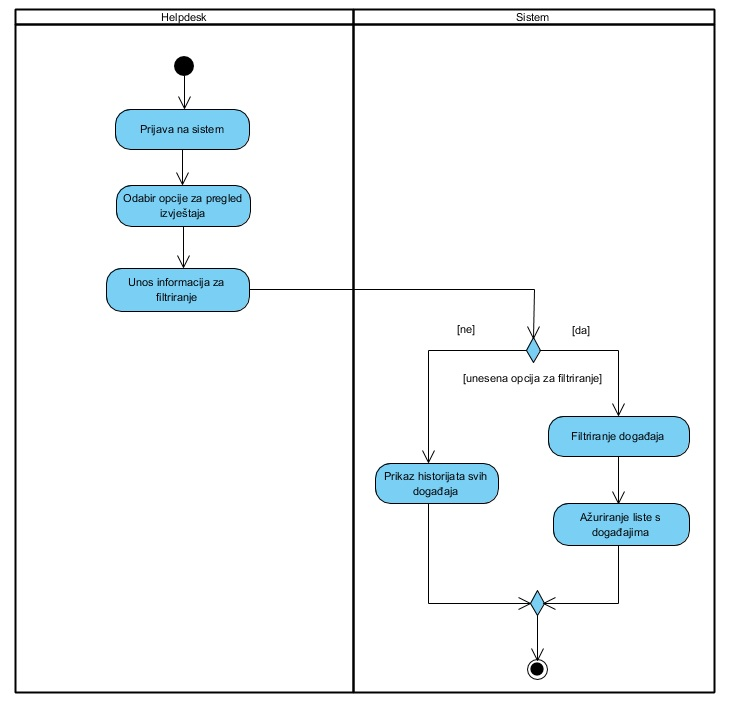
\includegraphics[scale=0.5]{../res/Activity/activity12.JPG}
\caption{Proces pregleda izvještaja}
\label{act12}
\end{figure}

\subsubsection{Izlazi}

Izlaz iz sistema predstavlja prikaz adekvatnog izvještaja, u kojoj su prikazani samo događaji koje dati korisnik smije vidjeti.

\subsubsection{Prioritet realizacije}

Prioritet realizacije ovog funkcionalnog zahtjeva je nizak, jer je pregled izvještaja statičan i nema snažan utjecaj na funkcionisanje sistema.

\newpage

\section{Arhitekturalni \textit{stack}}

\subsection{Dijagram klase}

Najjednostavniji način za opis arhitekture sistema je putem dijagrama klasa, na kojem su vidljive najvažniji dijelovi modela (klase) i veze između njih (generalizacija i asocijacija - kompozicija ili agregacija). Ovaj dijagram prikazan je na Slici \ref{class}.

\begin{figure}[H]
\center
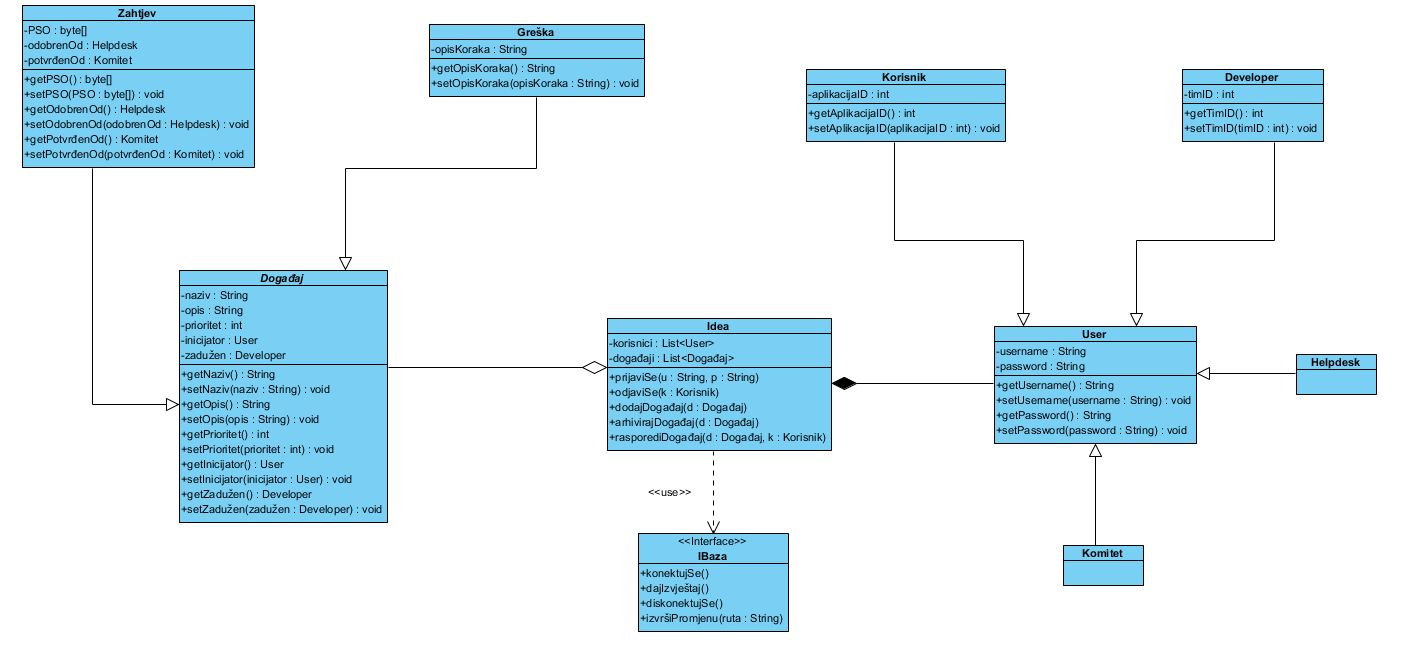
\includegraphics[scale=0.45]{../res/class.JPG}
\caption{Dijagram klasa sistema}
\label{class}
\end{figure}

\subsection{\textit{Entity Relationship} dijagram (ERD)}

Još jedan način za opis arhitekture sistema omogućen je putem \textit{entity relationship} dijagrama sistema, u kojem je prikazan model baze podataka koju sistem koristi. Ovaj dijagram prikazan je na Slici \ref{erd}.

\begin{figure}[H]
\center
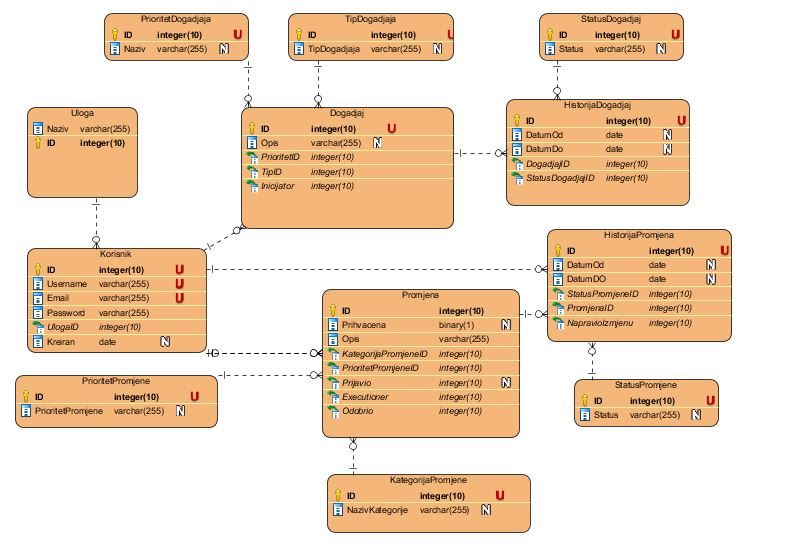
\includegraphics[scale=0.5]{../res/erd.JPG}
\caption{\textit{Entity relationship} dijagram sistema}
\label{erd}
\end{figure}

\newpage

\section{Tehnološki \textit{stack}}

\subsection{Opis korištenih tehnologija}

Pri razvoju sistema korištene su sljedeće tehnologije:

\begin{itemize}
\item \textbf{Frontend}: \\
\textit{Boostrap} za generisanje izgleda formi (koristeći HTML i CSS); \\
\textit{Angular framework} za izgradnju web-aplikacije;
\item \textbf{Backend}: \\
\textit{Node.js} tehnologija (programski jezik: \textit{JavaScript}); \\
\textit{MySQL} baza podataka;
\item \textbf{Dokumentacija}: \\
\textit{LaTex} za generisanje SRS dokumenta; \\
\textit{Visual Paradigm} za kreiranje UML dijagrama.
\end{itemize}

Tehnološki \textit{stack} sistema najlakše je predstaviti koristeći dijagram raspoređivanja, koji je prikazan na Slici \ref{deployment}. Na dijagramu je vidljivo da korisnik koristi \textit{interface}-e koje pruža \textit{frontend} dio sistema. \textit{Frontend} koristi servise backenda, a \textit{backend} jedini ima pristup bazi podataka. Na dijagramu je prikazano i koji dio sistema koristi koje od tehnologija koje su prethodno navedene.

\begin{figure}[H]
\center
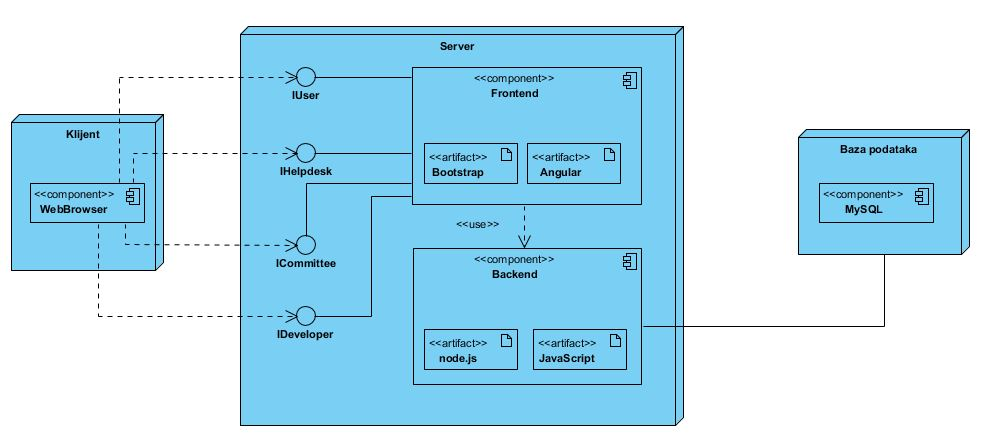
\includegraphics[scale=0.55]{../res/deployment.JPG}
\caption{Dijagram raspoređivanja sistema}
\label{deployment}
\end{figure}

\newpage

\section{Nefunkcionalni zahtjevi}

\subsection{Odziv sistema}

\quad Odziv sistema predstavlja količinu vremena od slanja zahtjeva do početka slanja odgovora sistema. Odziv sistema je veoma važna karakteristika za performanse sistema, te spor odziv (odnosno, dugo vrijeme odziva sistema) uzrokuje slabije performanse sistema. Vrijeme odziva sistema ovisi o mnogo faktora, a primarno o mogućnosti sistema da se nosi s velikim brojem korisnika bez da dođe do zagušenja mreže, te se zbog tog razloga hardverske komponente sistema trebaju prilagoditi na način da omogućavaju normalno funkcionisanje sistema i pri velikom broju zahtjeva od strane korisnika. \\

Budući da je sistem koji se razvija web-aplikacija koju će koristiti veliki broj, kako zaposlenika firme Idea, tako i kompanija za koje firma Idea razvija aplikacije, neophodno je da odziv sistema bude brz i u slučajevima kada u jednom trenutku bude poslan veliki broj zahtjeva (maksimalno 0.5 sekundi). Ovakav odziv omogućiti će se putem osposobljavanja više kopija istog servisa na koji će se preusmjeravati zahtjevi ovisno o stanju u redovima čekanja (koji trebaju biti približno isto napunjeni).

\subsection{Propusnost}

\quad Propusnost sistema se definiše kao količina informacija koje sistem može obraditi po jedinici vremena, te je također veoma važna za performanse sistema. Ona ovisi o mnogo faktora, uključujući brzinu procesiranja pojedinih informacija, kao i vrijeme odziva sistema, s kojim je propusnost direktno povezana. Budući da se propusnost odnosi na količinu informacija koje se mogu prenijeti preko mreže, pročitati ili napisati na medije za spašavanje podataka ili na broj operacija ulazno-izlaznih (I/O) uređaja, i propusnost sistema ovisi o više hardverskih komponenti, te je potrebno analizirati koja od naprijed navedenih propusnosti je esencijalna za funkcionisanje sistema te se analogno prilagoditi i hardverske komponente. \\

Propusnost sistema koji se razvija u vezi je s odzivom sistema koji je prethodno definisan - propusnost sistema treba biti velika (veliki broj istovremeno prijavljenih korisnika - najmanje 1,000 korisnika bez povećanja trajanja odziva), što će se omogućiti povećanjem kapaciteta redova čekanja, odnosno povećanjem broja redova čekanja (budući da je skaliranje u širinu jeftinije).

\subsection{Poruke o greškama}

\quad Za normalno funkcionisanje sistema potrebno je predvidjeti da korisnici neće uvijek na korektan način unositi tražene podatke i vršiti zadane operacije na ispravan način te se trebaju omogućiti poruke o greškama. Ukoliko korisnik napravi grešku, sistem istu treba prepoznati i prikazati korisniku adekvatne informacije kako bi se ponavljanje iste greške spriječilo. \\

Ovaj nefunkcionalni zahtjev ispunjen je tokom razvoja aplikacije, budući da je napravljen intuitivan korisnički \textit{interface} koji je jednostavan za korištenje. Tokom pokušaja prijave na sistem, ukoliko korisnik unese neispravne podatke, biti će mu prikazana adekvatna poruka. Ostatak sistema dizajniran je na način da se maksimalno izbjegnu greške pri unosu centriranjem na prikaz i \textit{button} kontrole umjesto na proizvoljan korisnički unos.

\subsection{Dostupnost}

\quad Dostupnost sistema definiše se kao vjerovatnoća da će poslani zahtjev od strane korisnika rezultovati odgovorom od strane sistema. Čak i mala količina vremena nedostupnosti sistema neprihvatljiva je (jer uzrokuje velike štete, što je dokazano u mnogim studijama) te se stoga treba osigurati da će sistem biti u stanju da uvijek ispravno funkcioniše, te ukoliko to ne bude moguće, da će se svaki kvar brzo i efikasno otkloniti od strane tima za održavanje, te da će korisnici biti obaviješteni kada i koliko dugo će sistem biti nedostupan (ukoliko je to moguće). \\

Dostupnost sistema također je u korelaciji s odzivom sistema, kao i s njegovom propusnošću, te još jednom potvrđuje neophodnost kreiranja većeg broja redundantnih kopija istih servisa - što više kopija istog servisa postoji, to je manja mogućnost da će u jednom trenutku sve dostupne kopije biti nedostupne, te da nijedan od servisa neće biti u mogućnosti odgovoriti na korisnički zahtjev. Kako bi se ovaj zahtjev ispunio, neophodno je da sistem bude dostupan 365 dana godišnje, s maksimalno 2 sata ukupne nedostupnosti.

\subsection{Skalabilnost}

\quad Skalabilnost je sposobnost sistema da se prilagođava sve većim zahtjevima u pogledu resursa i performansi. Pri dizajnu sistema i izbora hardverskih komponenti potrebno je uzeti u obzir informacije o broju korisnika koji će isti koristiti, vrsti usluga koje će sistem pružati te da li je potrebno omogućiti horizontalno ili vertikalno skaliranje (u skladu sa predviđenim budžetom). Budući da je pri dizajnu sistema korištena klijent-server arhitektura, skalabilnost je omogućena odvajanjem funkcionalnosti sistema u zasebne servise koji će se zasebno i skalirati (te time smanjiti i troškovi), te će sistem biti u stanju da funkcioniše i ukoliko jedna od komponenti ne bude funkcionisala (ili se bude nadograđivala), čime se direktno utječe i na dostupnost sistema. \\

Iako firma Idea ne planira da uskoro širi svoje poslovanje na veći broj firmi (jer je njena primarna djelatnost održavanje postojećih sistema), sistem koji se dizajnira svakako treba biti skalabilan, ukoliko se u budućnosti ipak odluči za ovakvo nešto. Skalabilnost je postignuta putem korištenja servis-klijent arhitekture sistema, koja omogućava dodavanje proizvoljnog broja kopija istog servisa, modifikaciju i nadogradnju određenih servisa bez utjecanja na ostale servise te čak i potpunu nezavisnost o operativnim sistemima koje korisnici koriste, budući da korisnik jedino treba posjedovati \textit{web-browser} kako bi pristupio sistemu.

\subsection{Dokumentovanost sistema}

\quad Za ispravno funkcionisanje sistema neophodno je da isti posjeduje što više što detaljnije dokumentacije, kako bi tim za održavanje u svakom trenutku mogao pronaći relevantne informacije za održavanje konkretnog servisa ili sistema kao cjeline. Osim dokumentacije za tim za održavanje, i korisnici trebaju imati adekvatnu dokumentaciju u obliku uputstava za korištenje, kako bi u svakom trenutku mogli pronaći relevantna uputstva za funkcionalnosti sistema koje žele koristiti.Uputstva za korištenje trebaju biti precizna i jasna, te koristiti terminologiju prilagođenu korisnicima sistema, kako ih ne bi zbunjivala te kako bi se rješenje nastalih problema pronašlo što brže i lakše. \\

Dokumentacija sistema predstavljena je u obliku SRS dokumenta, koji definiše sve bitne funkcionalnosti i ostale detalje o samom sistemu. U budućnosti je planirano i pravljenje korisničkog priručnika, kako bi korisnici mogli pronaći odgovore na sva eventualna pitanja i rješenja za sve nedoumice pri korištenju sistema.

\subsection{Autorizacija korisnika}

\quad Pristup neautorizovanim korisnicima treba biti onemogućen, te se iz tog razloga pri ulasku u sistem korisnici trebaju autorizovati, a to će uraditi putem unošenja ispravnih i jedinstvenih korisničkih podataka za koje će se izvršiti provjera unutar sistema. Ukoliko se uneseni korisnički podaci pronađu u sistemu, korisniku će biti omogućen pristup istom, te ukoliko se uneseni korisnički podaci ne pronađu u sistemu, korisniku će se prikazati poruka o neuspješnoj prijavi bez omogućavanja korištenja većine funkcionalnosti sistema. \\

Problem autorizacije u sistemu riješen je koristeći korisničke uloge i sesije. Postoji predefinisano vrijeme nakon kojeg se korisnik automatski odjavljuje iz sistema, kako bi se smanjila mogućnost zloupotrebe ukoliko se korisnik zaboravi odjaviti sistema. Rute sistema nisu blokirane na način da su samo sakriveni putevi koji vode do stranica za različite vrste korisnika, već se pri pristupu svakoj stranici provjerava uloga korisnika te se pristup dopušta isključivo ukoliko je korisnik autorizovan za pristup. Šifre korisnika u bazi podataka se čuvaju \textit{hash}-irane, tako da eventualno vršenje \textit{SQL Injections} neće ugroziti sigurnost korisnika.

\newpage

\section{Korisnički \textit{interface}-i}

\subsection{Forme vidljive svim korisnicima}

Svim korisnicima omogućen je pregled informacija o firmi Idea. To uključuje prikaz osnovnih informacija o firmi (prikazana na Slici \ref{s1}), detalja o načinu poslovanja (prikazana na Slici \ref{s2}), korisničkih iskustava (prikazana na Slici \ref{s3}) te mogućnost kontaktiranja firme od strane zainteresovanih korisnika (prikazana na Slici \ref{s4}). Svim korisnicima omogućen je i pristup formi \textbf{Login}, nakon što se klikne na dugme u gornjem desnom uglu aplikacije.

\begin{figure}[H]
\center

\includegraphics[scale=0.35]{../res/UI/home.PNG}
\caption{Izgled početne stranice}
\label{s1}
\end{figure}

\begin{figure}[H]
\center
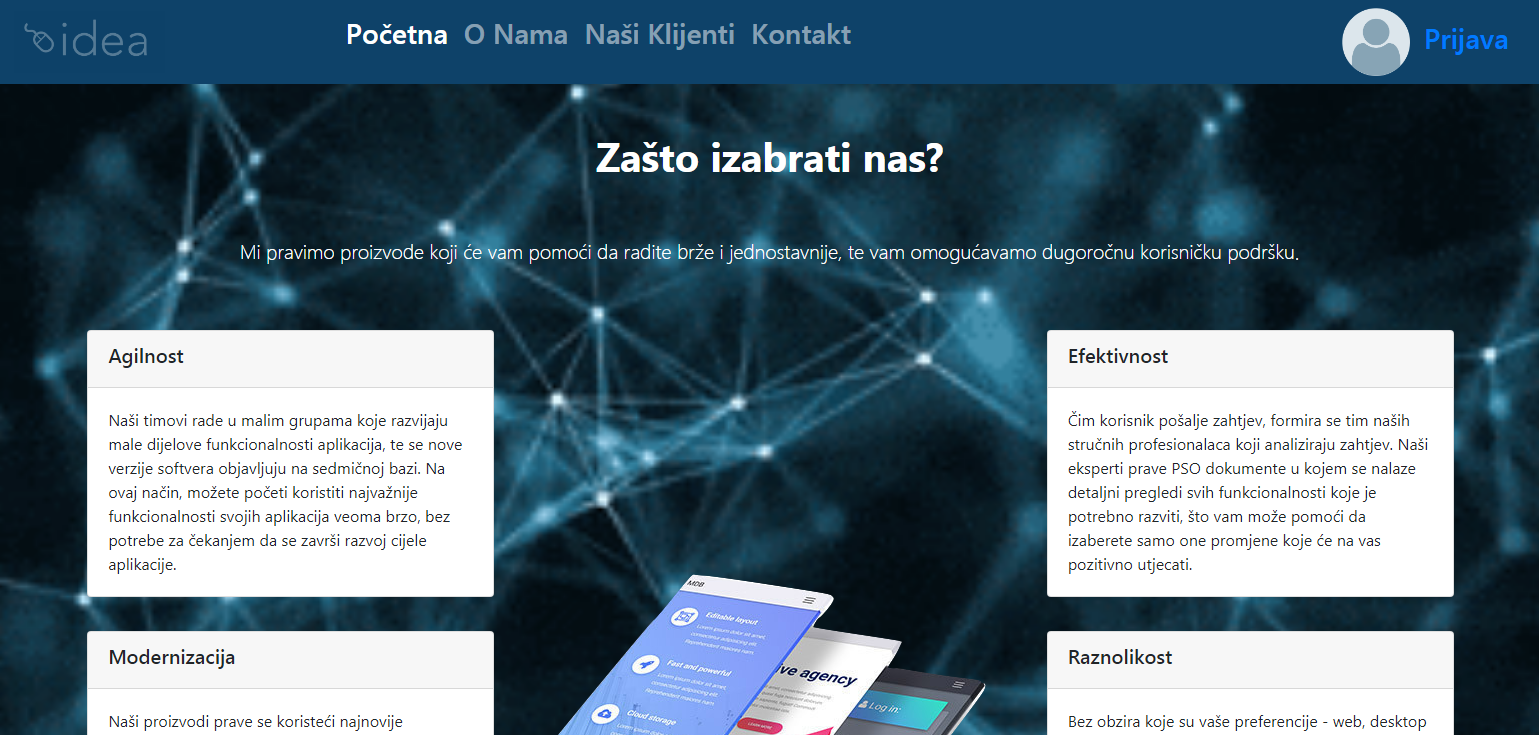
\includegraphics[scale=0.35]{../res/UI/about.PNG}
\caption{Detalji o firmi Idea}
\label{s2}
\end{figure}

\begin{figure}[H]
\center

\includegraphics[scale=0.35]{../res/UI/clients.PNG}
\caption{Pregled korisničkih iskustava}
\label{s3}
\end{figure}

\begin{figure}[H]
\center
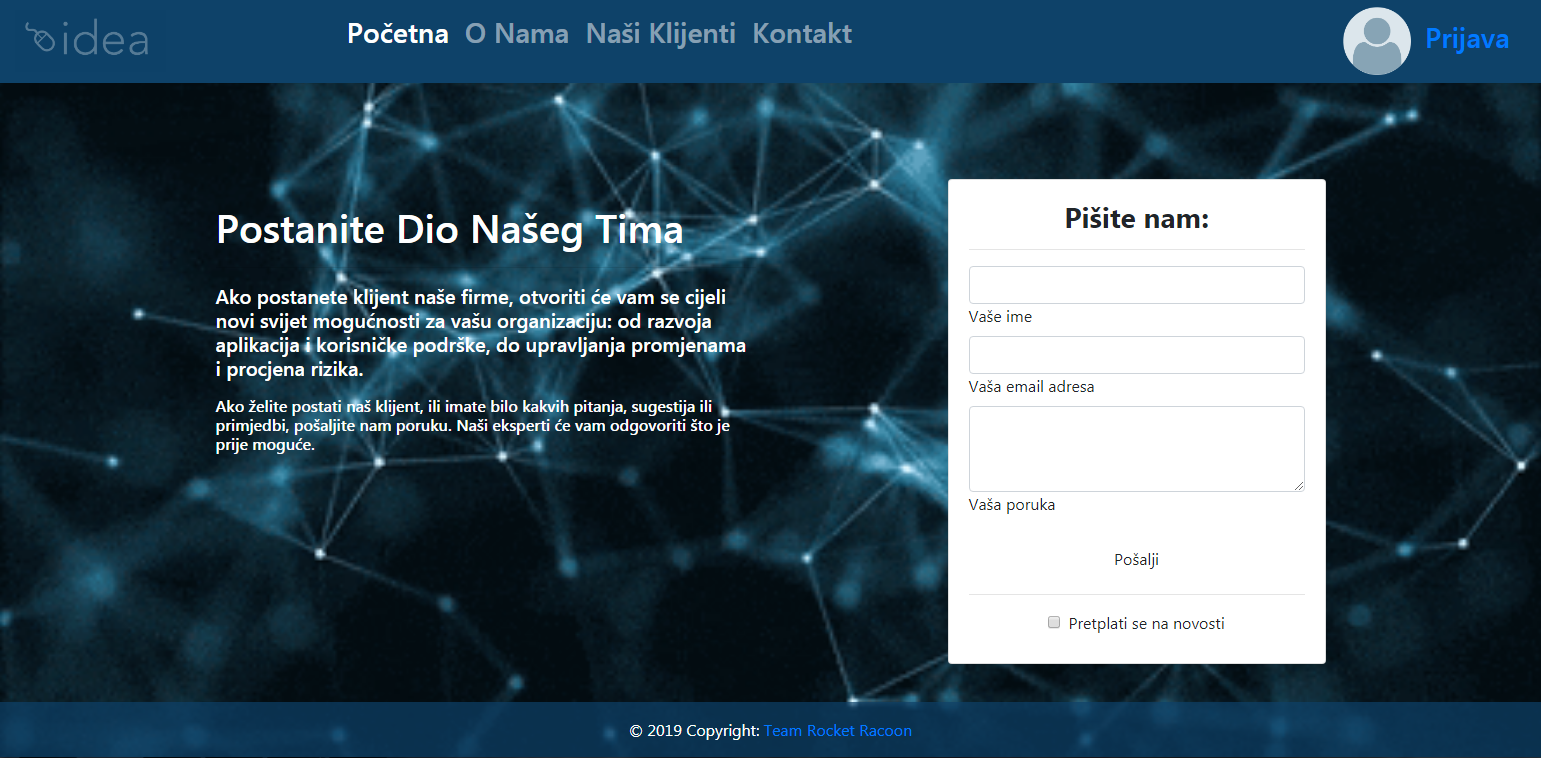
\includegraphics[scale=0.35]{../res/UI/contact.PNG}
\caption{Forma za kontaktiranje firme Idea}
\label{s4}
\end{figure}

Forma za prijavu zapravo je \textit{pop-up} koji omogućava korisnicima unos korisničkog imena i korisničke šifre (koje dodjeljuje tehnički administrator sistema, jer i korisnici sistema, a i osobe koje ga razvijaju i poboljšavaju, moraju imati neophodnu autorizaciju za pristup sistemu, budući da se u njemu nalaze osjetljivi podaci o javnim ustanovama, softveru koji se razvija, te dokumentima koje koristi komitet za promjene). \\

Forma za prijavu prikazana je na Slici \ref{s5}. Na Slici \ref{s6} prikazan je izgled forme nakon neuspješne prijave korisnika, odakle je vidljivo da poruke o greškama pri validaciji nisu napadne niti zbunjujuće, već da je korisniku omogućen jednostavan i intuitivan unos traženih podataka te lak pristup sistemu.

\begin{figure}[H]
\center
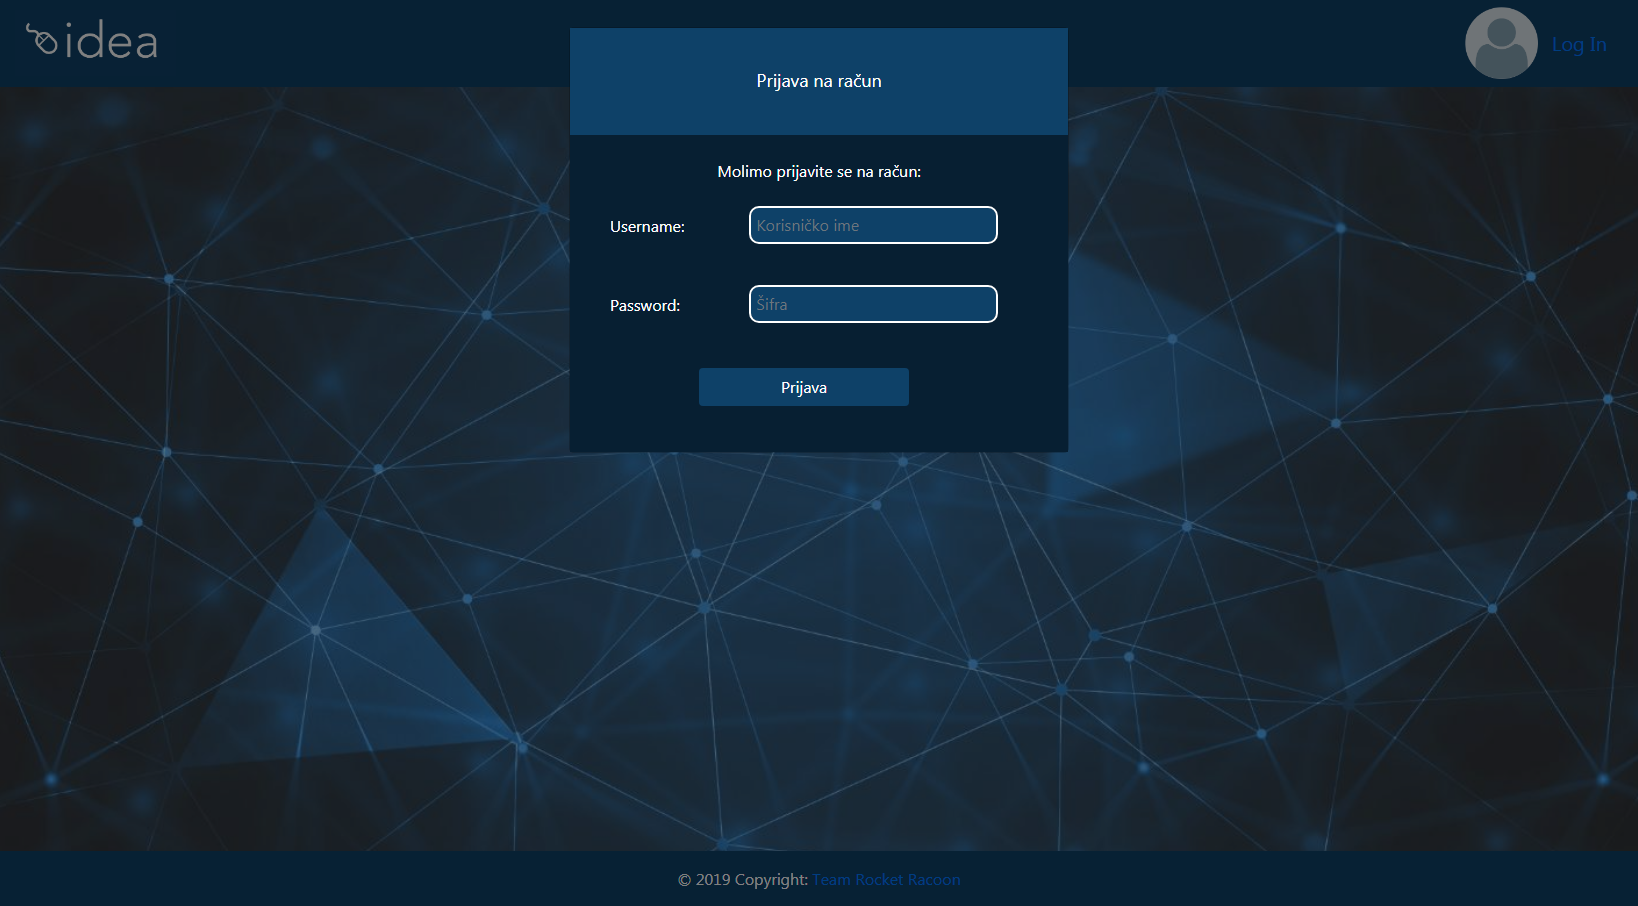
\includegraphics[scale=0.35]{../res/UI/login.PNG}
\caption{Izgled \textit{pop-up}-a za prijavu korisnika}
\label{s5}
\end{figure}

\begin{figure}[H]
\center
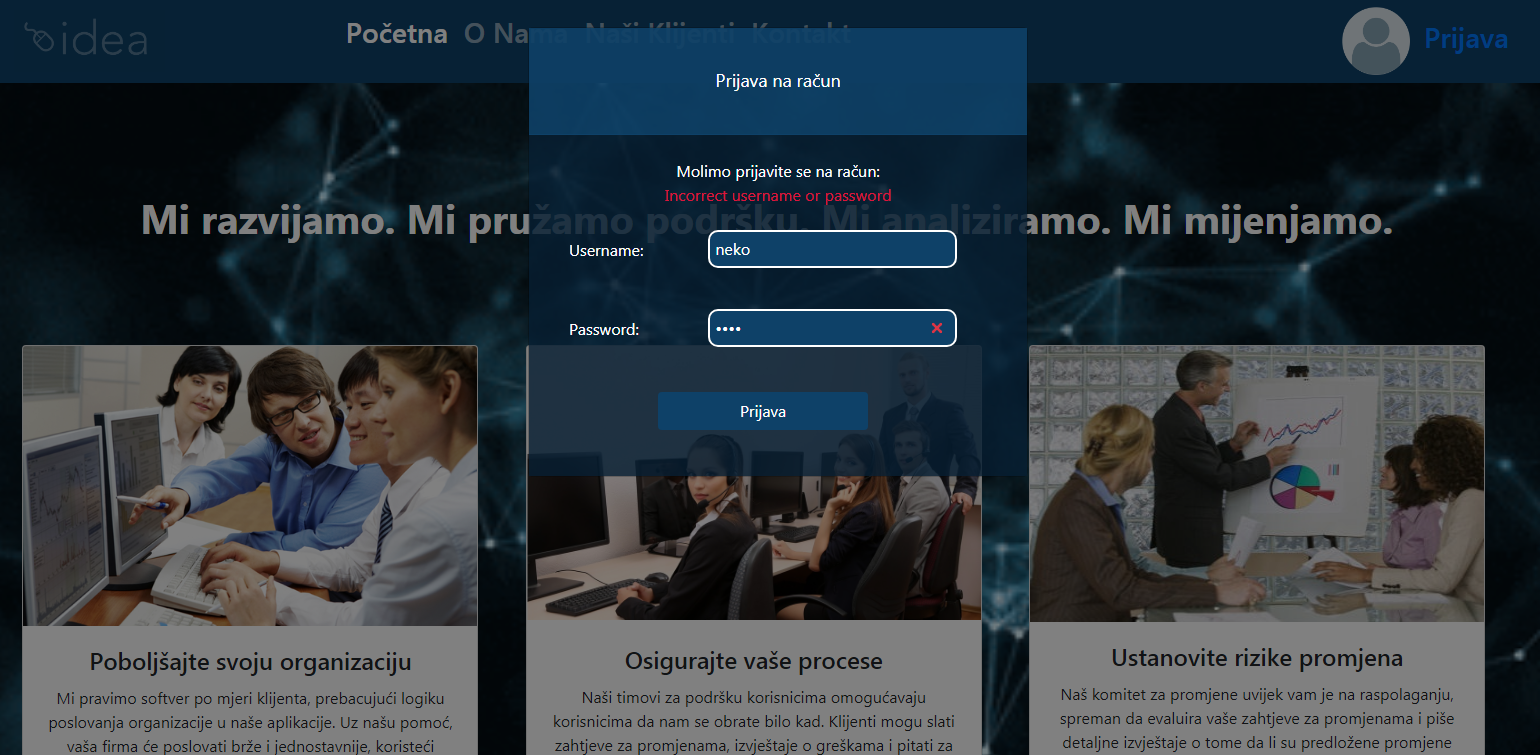
\includegraphics[scale=0.35]{../res/UI/loginFailed.PNG}
\caption{Izgled poruke o neuspješnoj validaciji}
\label{s6}
\end{figure}

\newpage

\subsection{Zahtjevi za promjenama}

Nakon prijave na sistem, različitim vrstama korisnika vidljiv je različit prikaz zahtjeva za promjenama:

\begin{enumerate}
\item Prikaz svih zahtjeva za promjenama (\textit{helpdesk});
\item Prikaz zahtjeva za promjenama koje je korisnik prijavio (korisnik softvera);
\item Prikaz zahtjeva za promjenama koje je \textit{helpdesk} dodijelio (komitet za promjene).
\end{enumerate}

Sama forma za prikaz ista je za sve različite vrste korisnika koje joj mogu pristupiti. Na njoj su prikazani samo aktuelni zahtjevi za promjenama. Izgled ove forme prikazan je na Slici \ref{s7}.

\begin{figure}[H]
\center
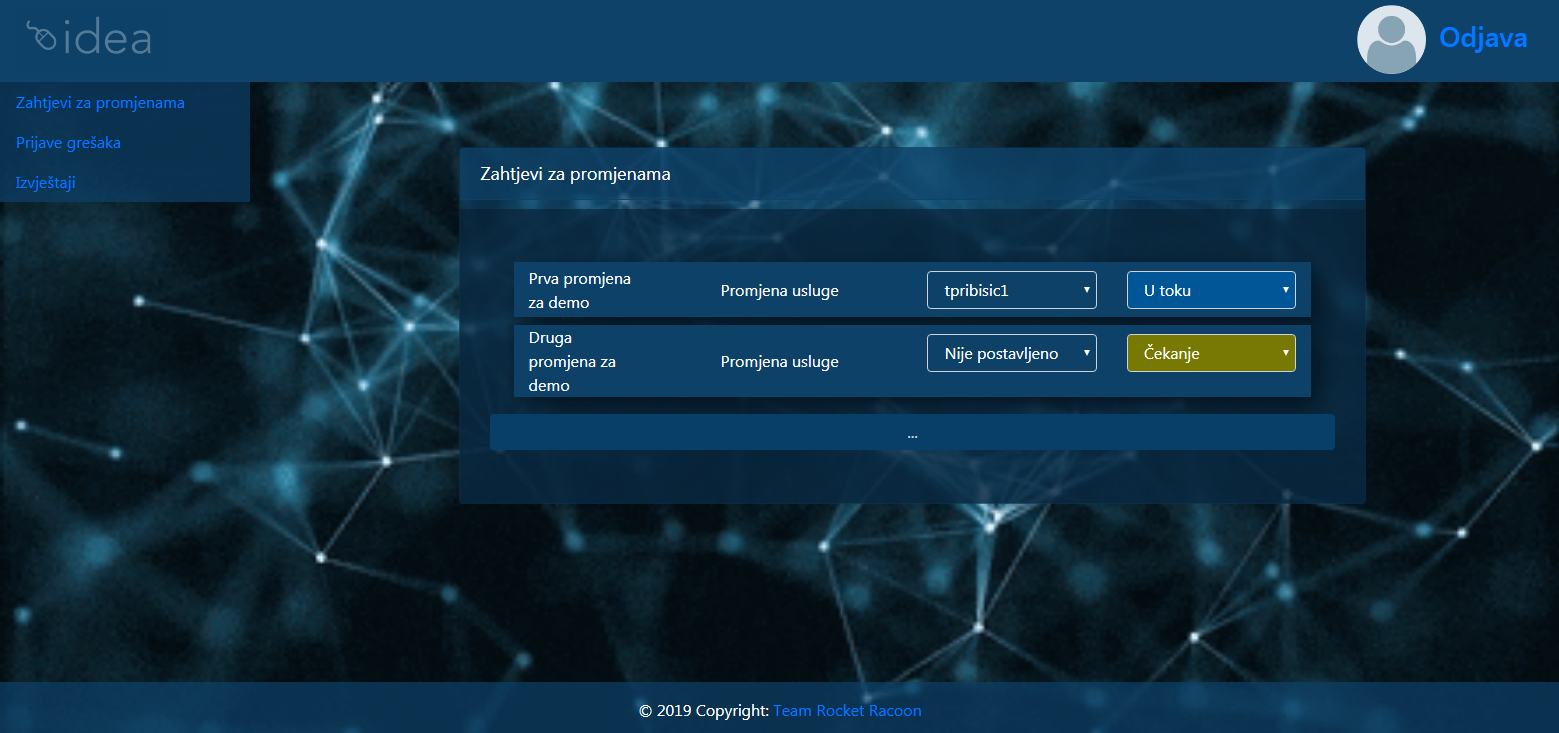
\includegraphics[scale=0.35]{../res/UI/changeActual.PNG}
\caption{Prikaz aktuelnih promjena}
\label{s7}
\end{figure}

Mogući statusi događaja su:

\begin{enumerate}
\item \textbf{Čekanje}: događaj nije raspoređen;
\item \textbf{U toku}: događaj je raspoređen (poslan timu za razvoj na implementaciju);
\item \textbf{Greška}: razvojni tim je prijavio grešku pri implementaciji promjene, te je neophodno hitno započeti s rješavanjem nastalog problema (koji može rezultovati promjenom specifikacije zahtjeva, ili odbacivanjem promjene);
\item \textbf{Završeno}: promjena je uspješno implementirana, te je potrebno izvršiti izdavanje nove verzije sistema i njegovo ažuriranje u skladu sa standardnom procedurom.
\end{enumerate}

Nakon klika na dugme \texttt{...}, korisniku je omogućen pregled svih zahtjeva za promjenama, kao što je prikazano na Slici \ref{s8}.

\begin{figure}[H]
\center
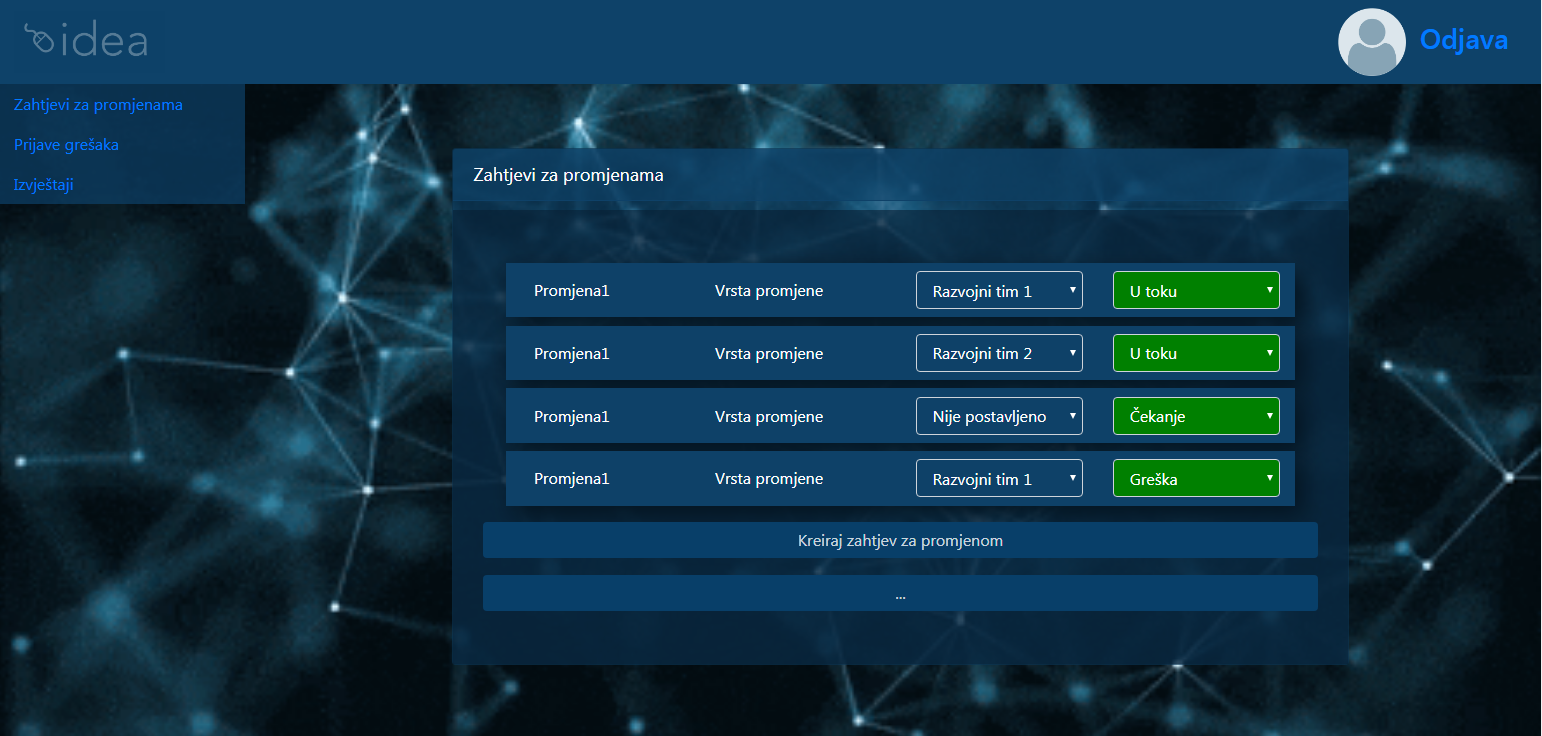
\includegraphics[scale=0.35]{../res/UI/changeAll.PNG}
\caption{Prikaz svih promjena}
\label{s8}
\end{figure}

Omogućen je prikaz i detalja o pojedinačnim promjenama, klikom na samu promjenu, nakon čega se na formi prikazuju sve relevantne informacije o nekoj promjeni (prikazano na Slici \ref{s9}).

\begin{figure}[H]
\center
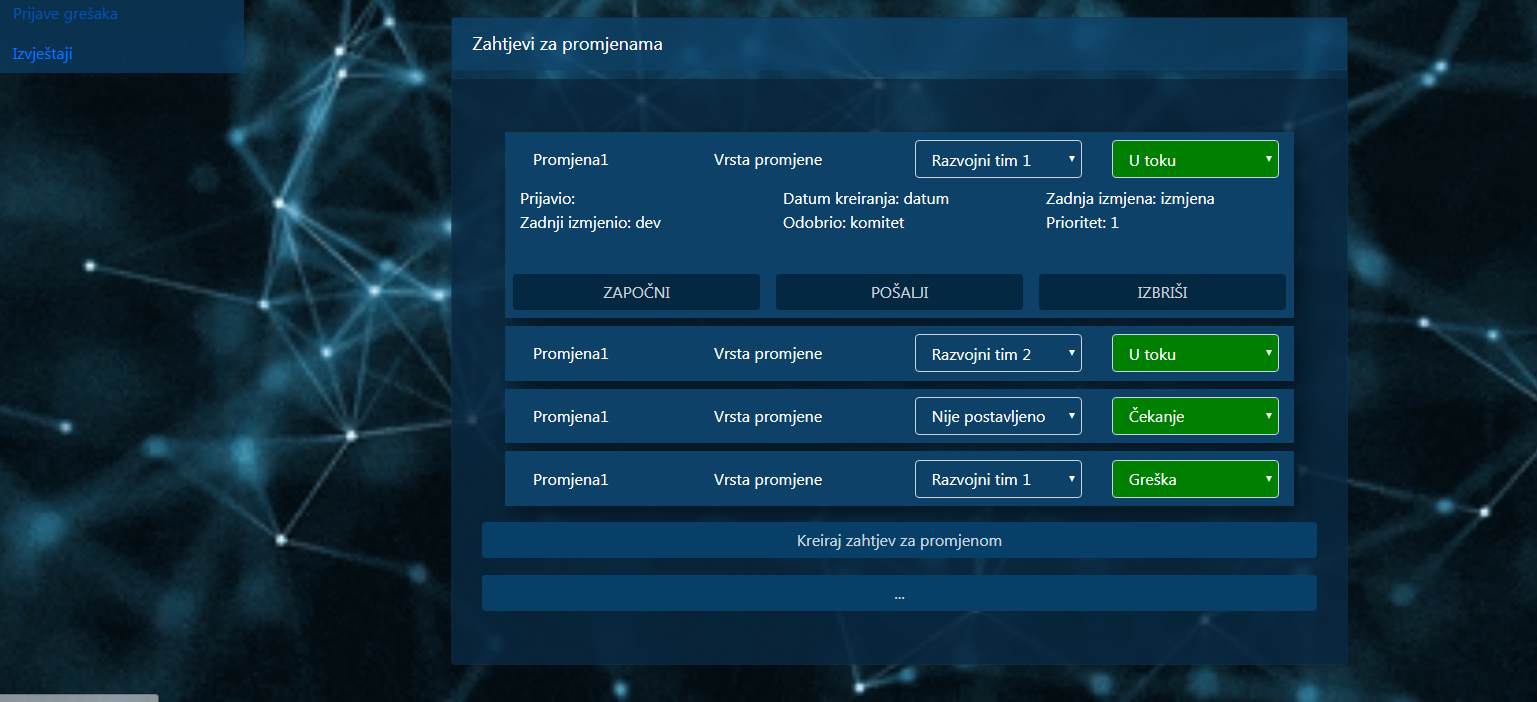
\includegraphics[scale=0.35]{../res/UI/changeDetails.PNG}
\caption{Prikaz detalja o promjeni}
\label{s9}
\end{figure}

Osim pregleda promjena i detalja o istim, moguće je i poslati novi zahtjev za promjenom, klikom na dugme \texttt{Kreiraj zahtjev za promjenom}. Nakon toga omogućava se unos podataka o promjeni, kao što je prikazano na Slici \ref{s10}.

\begin{figure}[H]
\center
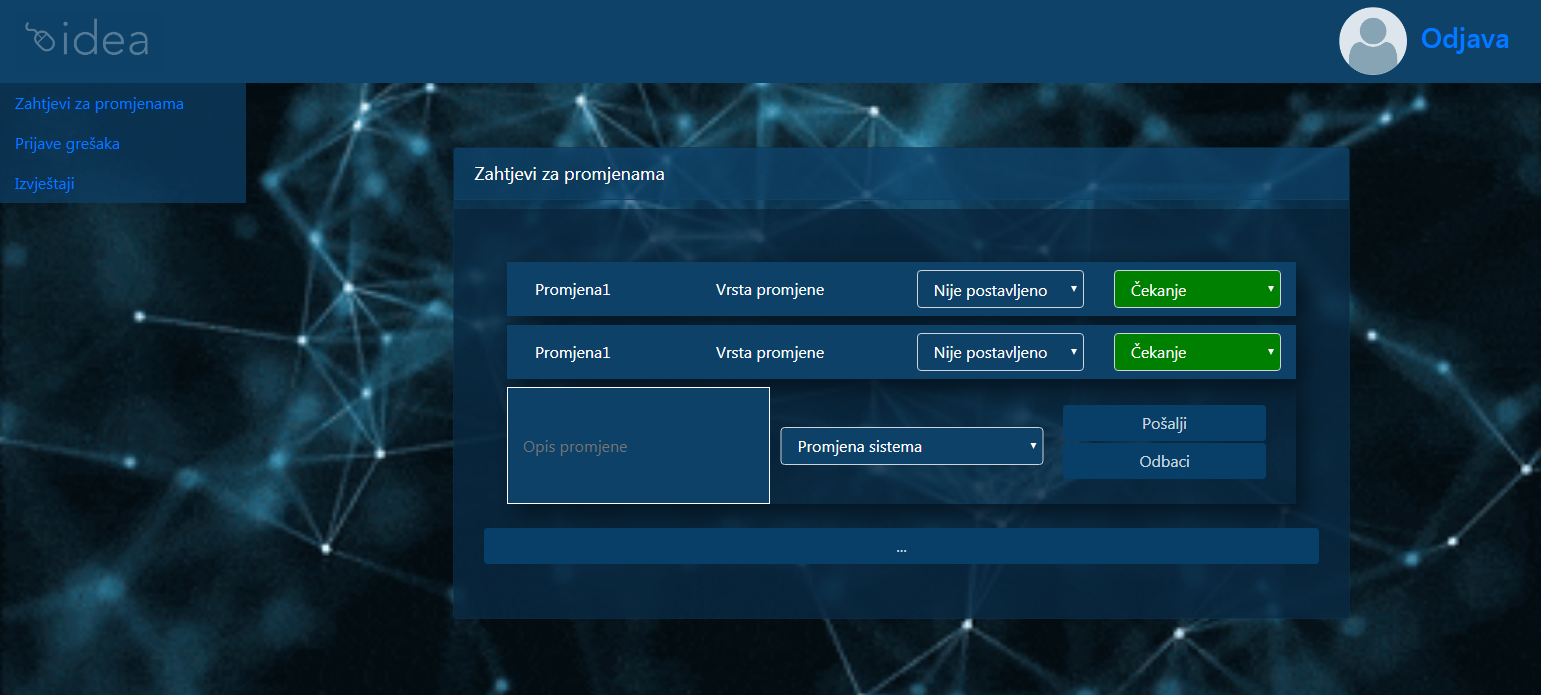
\includegraphics[scale=0.35]{../res/UI/changeAdd.PNG}
\caption{Mogućnost dodavanja novog zahtjeva za promjenom}
\label{s10}
\end{figure}

\newpage

\subsection{Prijave grešaka}

Nakon prijave na sistem, različitim vrstama korisnika vidljiv je različit prikaz prijava grešaka:

\begin{enumerate}
\item Prikaz svih prijava grešaka (\textit{helpdesk});
\item Prikaz grešaka koje je korisnik prijavio (korisnik softvera);
\item Prikaz grešaka koje je \textit{helpdesk} dodijelio (razvojni tim).
\end{enumerate}

Sama forma za prikaz ista je za sve različite vrste korisnika koje joj mogu pristupiti. Na njoj su prikazani samo aktuelne prijave grešaka. Izgled ove forme prikazan je na Slici \ref{s11}.

\begin{figure}[H]
\center
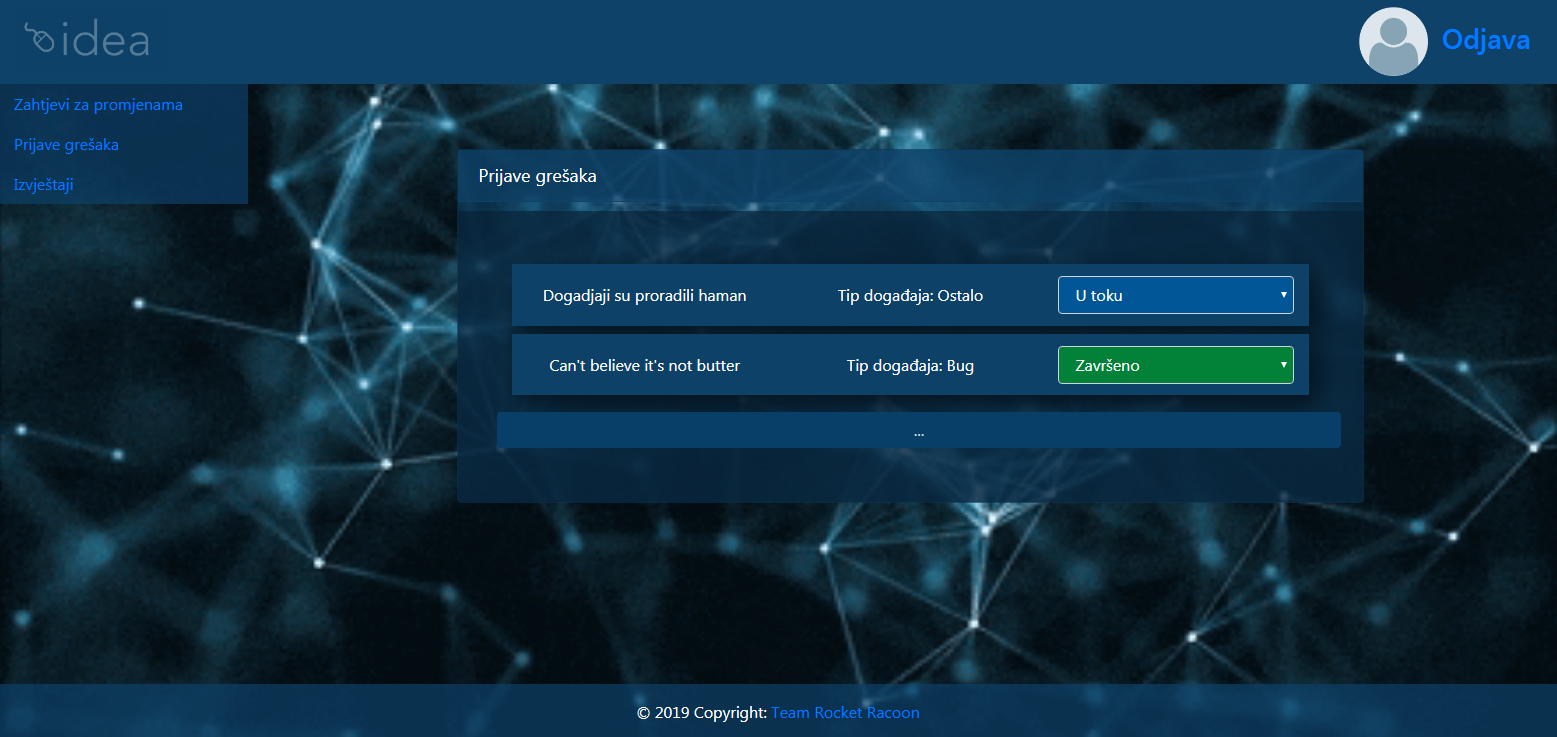
\includegraphics[scale=0.35]{../res/UI/errorActual.PNG}
\caption{Prikaz aktuelnih prijava grešaka}
\label{s11}
\end{figure}

Način na koji se tretiraju greške pri implementiranju promjena i \textit{bug}-ovi otkriveni nakon uvođenja promjena fundamentalno je različit, te je opisan kako slijedi:
\begin{enumerate}
\item Ukoliko član razvojnog tima prijavi \textbf{grešku pri implementaciji promjene}, odnosno ukoliko razvojni tim prijavi da iz nekog razloga u postojeći sistem ne može inkorporisati zahtjev za promjenom koji je ocijenjen kao isplativ i odobren za razvoj, \textit{helpdesk} je dužan odmah izvršiti reviziju PSO dokumenta, dodatno se konsultovati s komitetom te da donijeti konačnu odluku o odbacivanju zahtjeva ili promjeni specifikacije zahtjeva na osnovu koje se vrši implementacija promjene;
\item Ukoliko korisnik aplikacije prijavi \textbf{\textit{bug}} u aplikaciji (sam način prijave biti će detaljnije opisan u narednom poglavlju), \textit{helpdesk} ne dobiva nikakvu notifikaciju, no lista svih \textit{bug}-ova (kojoj samo razvojni tim ima pristup) ažurira se na način da se prijava dodaje u listu kao novi unos. Unosi iz te liste svakodnevno se pokušavaju riješiti i lista se svakodnevno ažurira u ovisnosti o ispravljenim \textit{bug}-ovima (mada tim za razvoj mora odlučiti da li je prijavljeni \textit{bug} uopće zaista greška u aplikaciji, te ukoliko nije, unos je moguće obrisati iz liste jednostavnim odbacivanjem \textit{bug}-a).
\end{enumerate}

Nakon klika na dugme \texttt{...}, korisniku je omogućen pregled svih prijava grešaka, kao što je prikazano na Slici \ref{s12}.

\begin{figure}[H]
\center
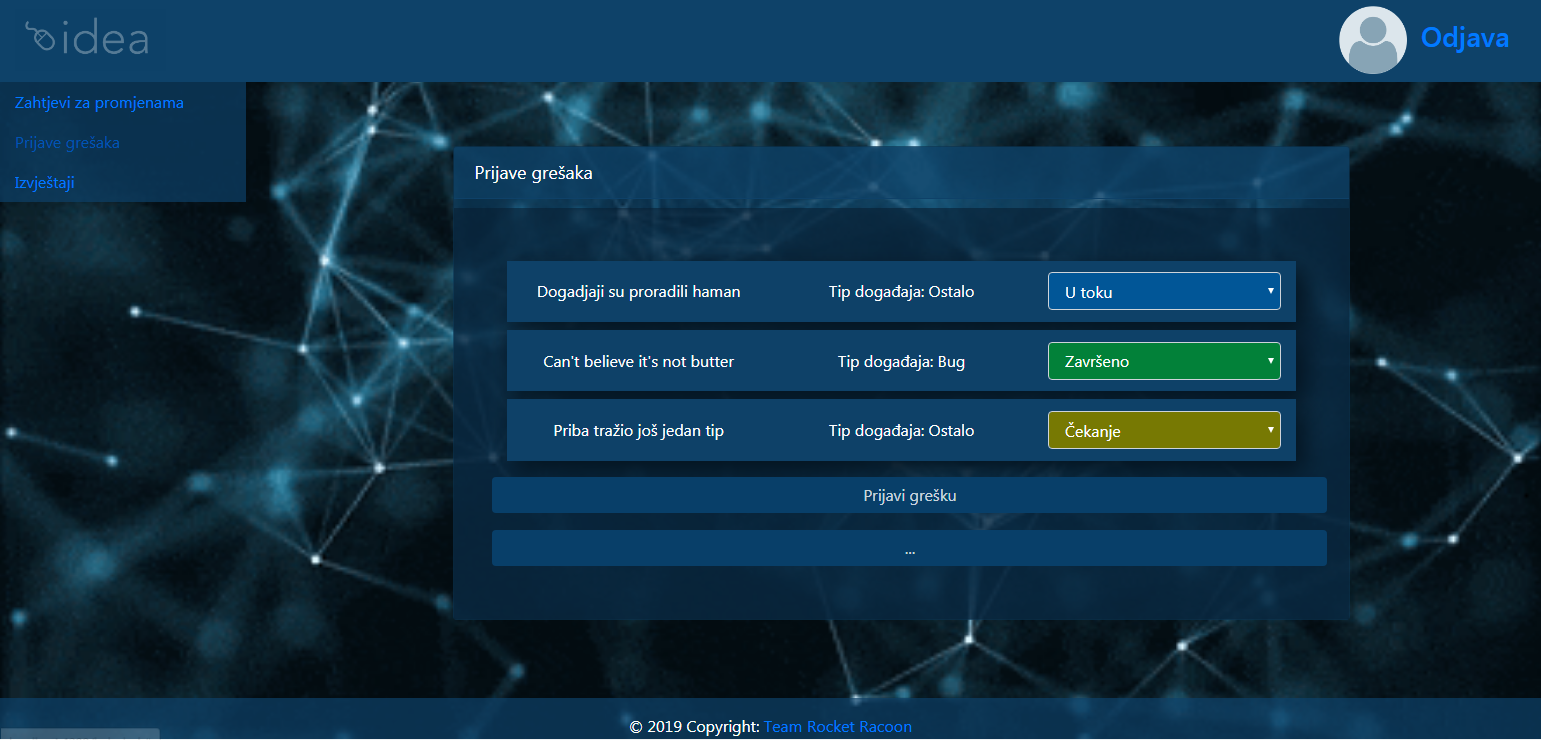
\includegraphics[scale=0.35]{../res/UI/errorAll.PNG}
\caption{Prikaz svih prijava grešaka}
\label{s12}
\end{figure}

Omogućen je prikaz i detalja o pojedinačnim prijavama, klikom na samu prijavu, nakon čega se na formi prikazuju sve relevantne informacije o nekoj prijavi (prikazano na Slici \ref{s13}).

\begin{figure}[H]
\center
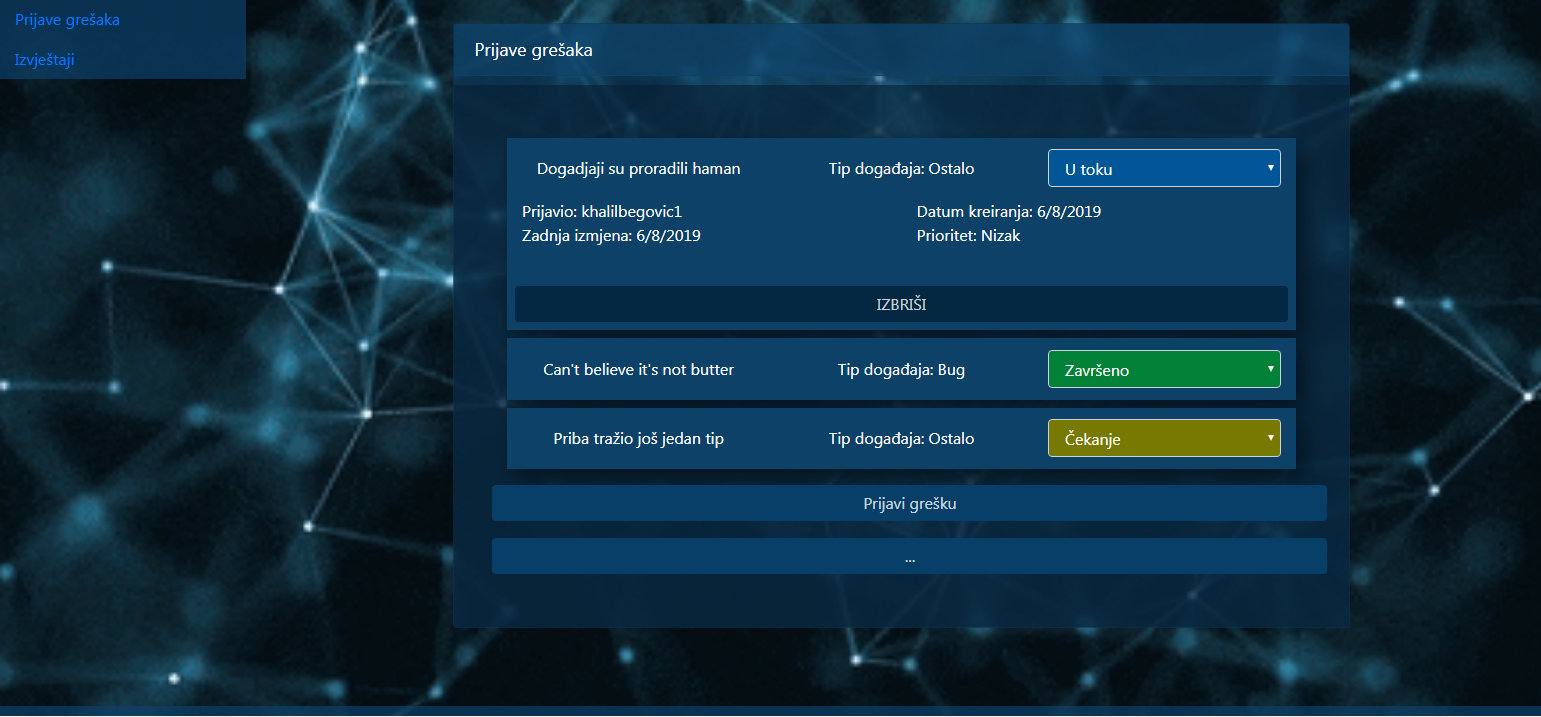
\includegraphics[scale=0.35]{../res/UI/errorDetails.PNG}
\caption{Prikaz detalja o prijavi greške}
\label{s13}
\end{figure}

Osim pregleda prijava i detalja o istim, moguće je i prijaviti novu grešku, klikom na dugme \texttt{Prijavi grešku}. Nakon toga omogućava se unos podataka o prijavi, kao što je prikazano na Slici \ref{s14}.

\begin{figure}[H]
\center
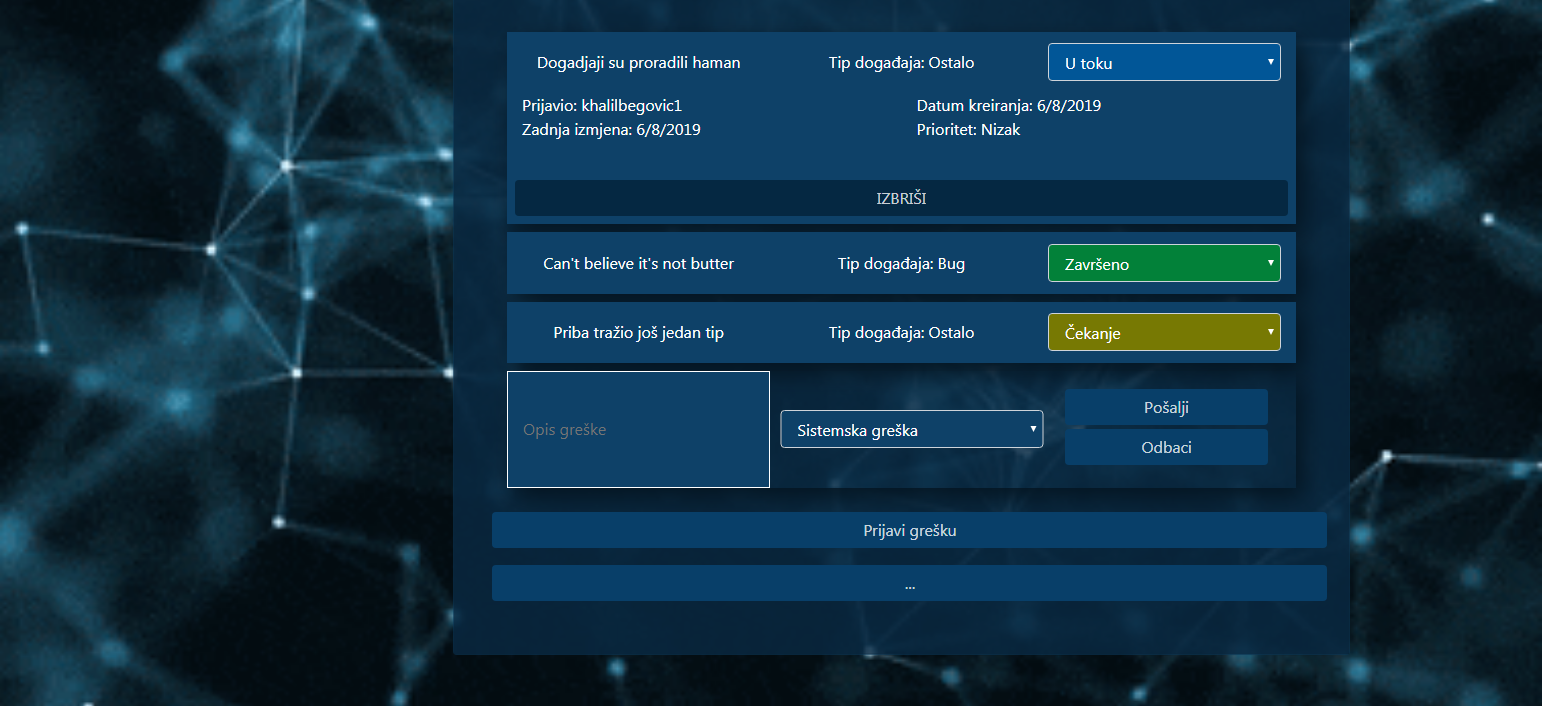
\includegraphics[scale=0.35]{../res/UI/errorAdd.PNG}
\caption{Mogućnost prijave nove greške}
\label{s14}
\end{figure}

\newpage

\subsection{Izvještaji}

Različite vrste korisnika imaju mogućnost pregleda različitih izvještaja:

\begin{enumerate}
\item \textit{Helpdesk}: prikaz cjelokupnog izvještaja o cijelom sistemu;
\item \textit{Ostali korisnici}: prikaz izvještaja s podacima samo o onim dijelovima sistema koji su vidljivi datom korisniku.
\end{enumerate}

Cjelokupni izvještaj uključuje prikaz svih korisnika, te prikaza svih detalja o svim promjenama i greškama, te njihovim promjenama i fazama kroz koje su pojedinačne promjene i greške prolazile u toku svoje aktivnosti, kao što je prikazano na Slici \ref{s15}, \ref{s16}, \ref{s17}, \ref{s18} i \ref{s19}. Ovakav prikaz neophodan je \textit{helpdesk}-u, za praćenje svih događaja u sistemu. Ostalim korisnicima omogućen je prikaz samo promjena, odnosno grešaka koje su prijavili ili koje su im dodijeljene.

\begin{figure}[H]
\center
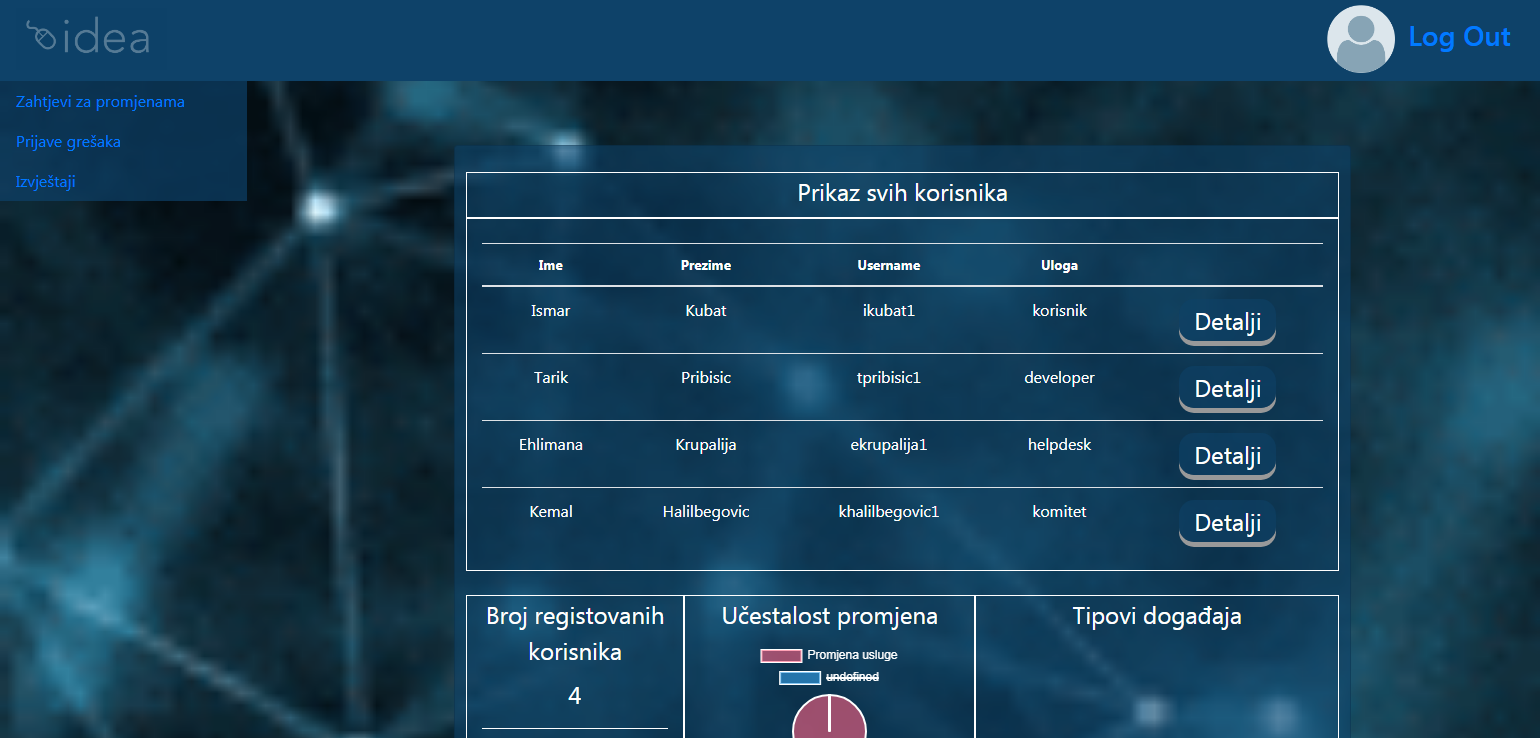
\includegraphics[scale=0.35]{../res/UI/report1.PNG}
\caption{Prikaz kompletnog izvještaja - korisnici}
\label{s15}
\end{figure}

\begin{figure}[H]
\center
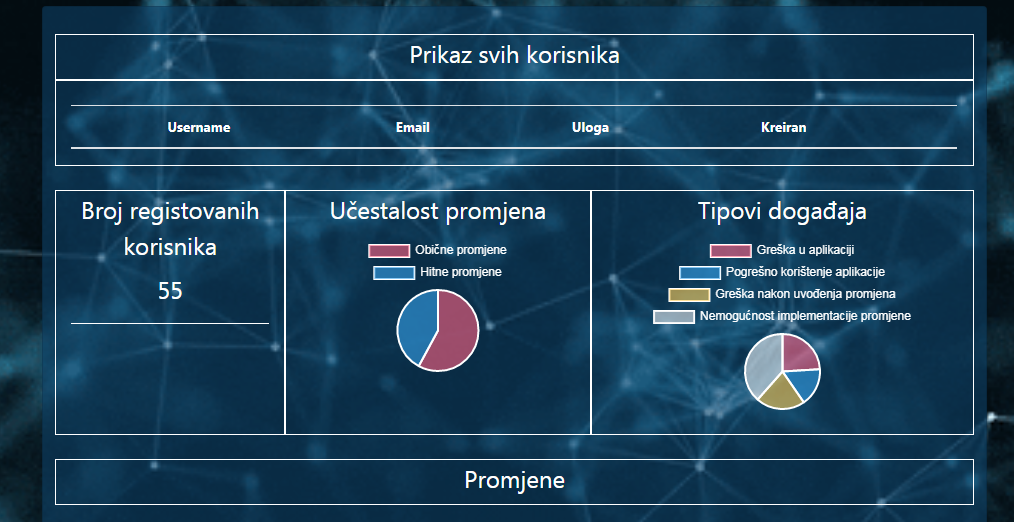
\includegraphics[scale=0.4]{../res/UI/report1-1.PNG}
\caption{Prikaz kompletnog izvještaja - statistika o korisnicima}
\label{s16}
\end{figure}

\begin{figure}[H]
\center
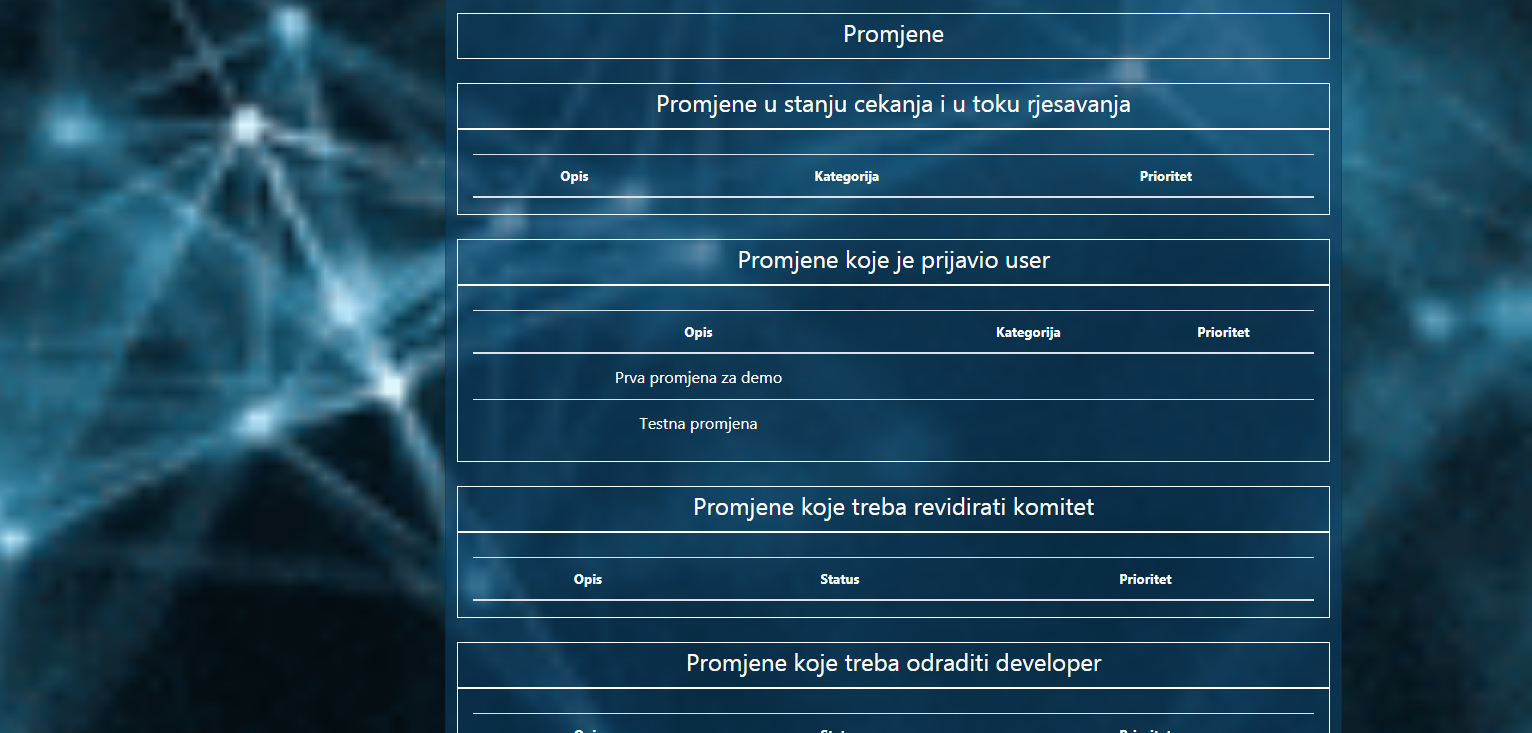
\includegraphics[scale=0.35]{../res/UI/report2.PNG}
\caption{Prikaz kompletnog izvještaja - promjene (prvi dio)}
\label{s17}
\end{figure}

\begin{figure}[H]
\center
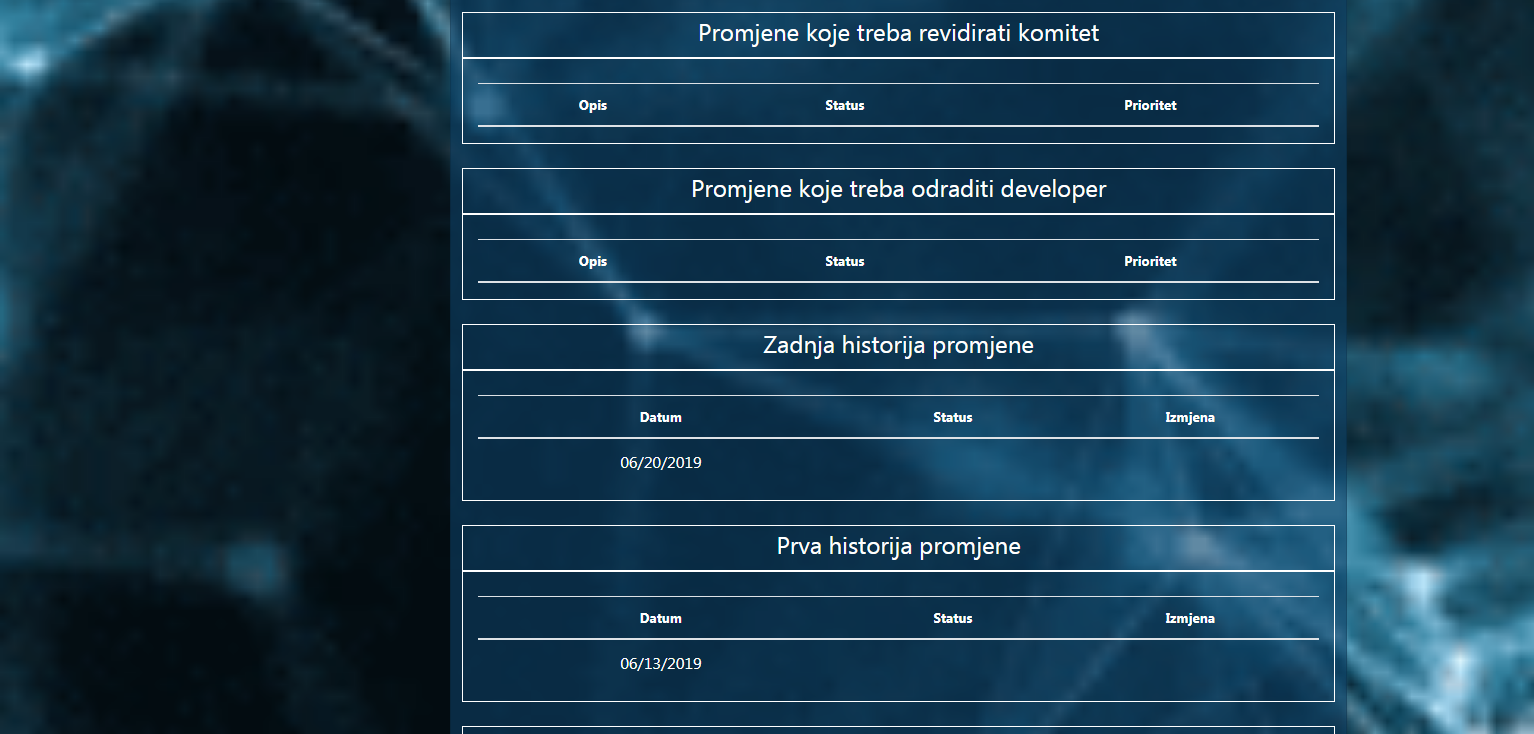
\includegraphics[scale=0.35]{../res/UI/report3.PNG}
\caption{Prikaz kompletnog izvještaja - promjene (drugi dio)}
\label{s18}
\end{figure}

\begin{figure}[H]
\center
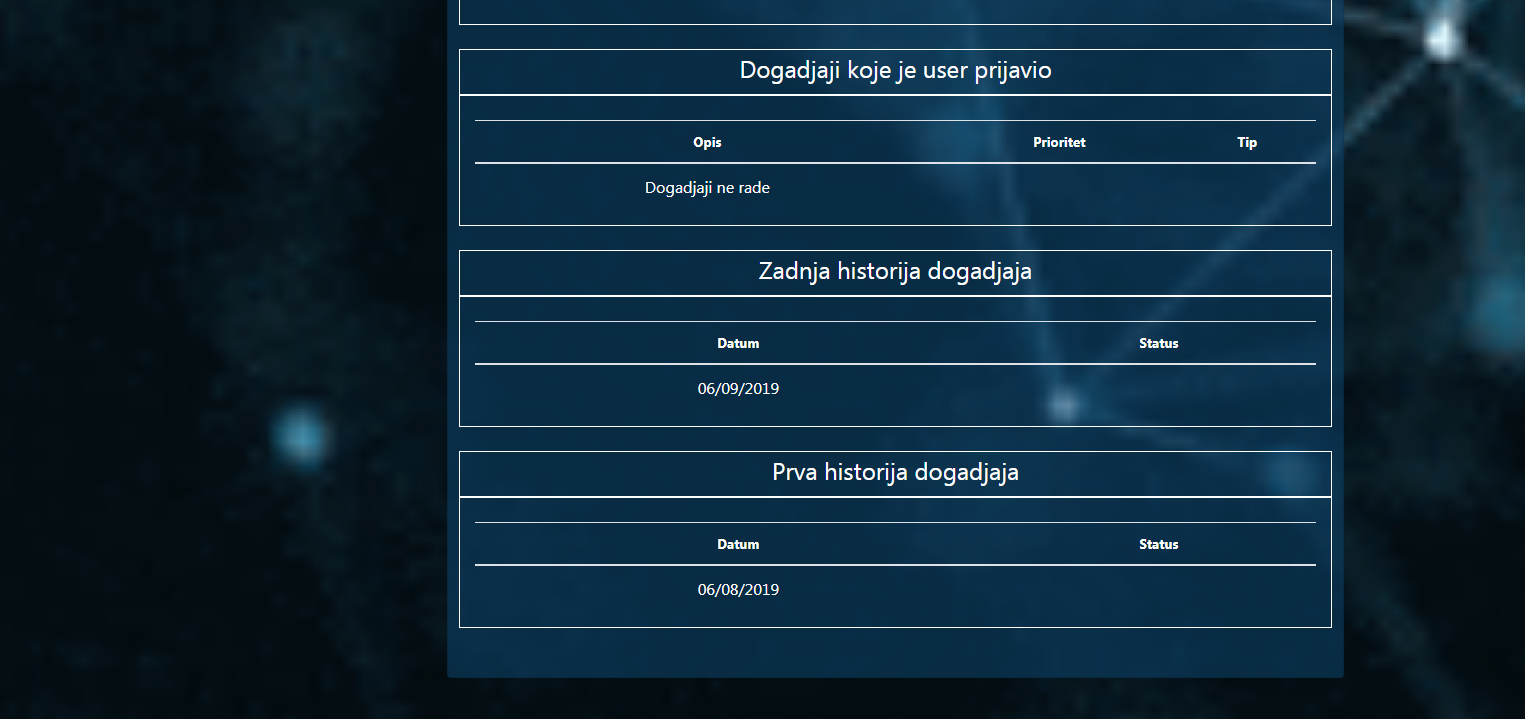
\includegraphics[scale=0.35]{../res/UI/report4.PNG}
\caption{Prikaz kompletnog izvještaja - događaji}
\label{s19}
\end{figure}

\newpage

\section{Zakonska ograničenja dizajna}

Sistem će biti razvijen u skladu s ograničenjima koja su propisana u sljedećim zakonima:

\begin{enumerate}
\item \textbf{Zakon o privrednim društvima Federacije Bosne i Hercegovine}: \\
\textit{Član 38.} Poslovnom tajnom smatraju se informacije o poslovanju za koje je očito da bi prouzrokovale značajnu štetu društvu ako dođu u posjed trećeg lica bez saglasnosti društva. \\
\textit{Član 39. (1)} Nadležni organ društva dužan je pismenim aktom odrediti informacije koje imaju karakter poslovne tajne i lica odgovorna za njihovo korištenje i zaštitu.
U skladu sa prethodno navedenim članom, zakonska ograničenja predstavljaju i svi pisani akti doneseni od strane vrtića, a kojima se definišu podaci za koje je potrebno onemogućiti pristup svim neovlaštenim licima. \\
Naprijed navedeni članovi (kao i svi pisani akti doneseni od strane firme Idea, a koji se odnose na podatke koje je potrebno zaštititi od neovlaštenog pristupa) postavljaju ograničenja pristupa različitih vrsta korisnika podacima za koje nisu ovlašteni. Budući da će razvijenoj aplikaciji biti u mogućnosti pristupiti osobe koje nisu zaposlenici firme Idea, sve podatke je potrebno zaštititi putem obavezne autorizacije pri pokušaja pristupa svim funkcionalnostima sistema.
\item \textbf{Zakon o zaštiti ličnih podataka Bosne i Hercegovine}:
\textit{Član 11. (1)} Kontrolor podataka i, u okviru svoje nadležnosti, obrađivač podataka staraju se o bezbjednosti podataka te preduzimaju sve tehničke i organizacione mjere i utvrđuju pravila postupka, koji su neophodni kako bi se sproveo ovaj zakon i drugi propisi u vezi sa zaštitom i tajnošću podataka. \\
\textit{Član 11. (2)} Kontrolor i obrađivač dužni su da preduzmu mjere protiv neovlašćenog ili slučajnog pristupa ličnim podacima, mijenjanja, uništavanja ili gubitka podataka, neovlašćenog prenosa, drugih oblika nezakonite obrade podataka, kao i mjere protiv zloupotrebe ličnih podataka. Ova obaveza ostaje na snazi i nakon završene obrade podataka. \\
Naprijed navedeni članovi postavljaju ograničenja na pristup podacima za korisnike sistema. Pregled korisnika će biti onemogućen te će biti poduzete sve mjere zaštite od krađe podataka korisnika (njihovih korisničkih imena i šifri, te svih ostalih reevantnih podataka) od strane zlonamjernih korisnika aplikacije. \\
\end{enumerate}

Dokument je napisan u skladu sa IEEE 830-1998 standardom (\textit{IEEE Recommended Practice for Software Requirements Specification}).

\end{document}